
\documentclass[12pt,a4paper]{report}

% ── Geometry and Layout ─────────────────────────────────────────
\usepackage[a4paper, top=20mm, bottom=20mm, left=20mm, right=20mm, headheight=52pt, headsep=12pt, footskip=30pt, includehead, includefoot]{geometry}

% ── Core Packages ─────────────────────────────────────────────
\usepackage{graphicx}
\usepackage{amsmath}
\usepackage{amssymb}
\usepackage{booktabs}
\usepackage{array}
\usepackage{tabularx}
\usepackage{float}
\usepackage{fancyhdr}
\usepackage[hidelinks]{hyperref}
\usepackage{xcolor}
\usepackage{setspace}
\usepackage{enumitem}
\usepackage{caption}
\usepackage{subcaption}
\usepackage{multirow}
\usepackage{colortbl}
\usepackage{longtable}
\usepackage{titlesec}
\usepackage{titletoc}
\usepackage{lastpage}
\usepackage{makecell}
\usepackage{etoolbox}
\usepackage{needspace}
\setlength{\emergencystretch}{2em}

% ── Color Definitions ─────────────────────────────────────────
\definecolor{osdagGreen}{HTML}{91B014}
\definecolor{osdagDarkGreen}{HTML}{64850C}
\definecolor{tableHeaderBg}{HTML}{EBF1D5}
\definecolor{tableRowZebra}{HTML}{F9FAF5}
\definecolor{tableBorder}{HTML}{B0C080}
\definecolor{urFailRed}{HTML}{D32F2F}
\definecolor{urPassGreen}{HTML}{2E7D32}

% Palettes SSOT
\definecolor{navyPrimary}{HTML}{1A365D}
\definecolor{steelBlue}{HTML}{2B6CB0}
\definecolor{charcoalText}{HTML}{2D3748}
\definecolor{zebraFill}{HTML}{F7FAFC}
\definecolor{borderRule}{HTML}{CBD5E0}
\definecolor{alertRed}{HTML}{E53E3E}
\definecolor{successGreen}{HTML}{38A169}

% ── Caption Styling ───────────────────────────────────────────
\captionsetup{
    labelfont=bf,
    justification=raggedright,
    singlelinecheck=false,
    format=plain
}

% ── Numbering and Floats ────────────────────────────────────────
\numberwithin{table}{chapter}
\numberwithin{figure}{chapter}

% ── Centralized Table Spacing and Geometry Rules ────────────────
\setlength{\tabcolsep}{6pt}
\renewcommand{\arraystretch}{1.18}
\setlength{\arrayrulewidth}{0.5pt}
\setlength{\extrarowheight}{1.0pt}
\setlength{\LTpre}{6pt}
\setlength{\LTpost}{6pt}
\setlength{\LTleft}{\fill}
\setlength{\LTright}{\fill}

% Buffer control: prevent orphan tables and margin bleed
\BeforeBeginEnvironment{table}{\Needspace{12\baselineskip}}
\BeforeBeginEnvironment{longtable}{\Needspace{12\baselineskip}}

% ── Running Headers and Footers ─────────────────────────────────
\fancypagestyle{main}{
  \fancyhf{}
  \fancyhead[L]{\parbox[b]{0.60\headwidth}{\raggedright\footnotesize\textsf{OsdagBridge report verification - synthetic fixture $|$ }}}
  \fancyhead[R]{\parbox[b]{0.36\headwidth}{\raggedleft\footnotesize\textsf{2026-11-11 $|$ Layout and data-mapping test; not a completed engineering design}}}
  \fancyfoot[L]{\footnotesize\textsf{Osdag $|$ FOSSEE $|$ Indian Institute of Technology Bombay}}
  \fancyfoot[R]{\footnotesize\textsf{Page \thepage\ of \pageref{LastPage}}}
  \renewcommand{\headrule}{\color{osdagGreen}\hrule width\headwidth height 1pt \vspace{2pt}}
  \renewcommand{\footrule}{%
    \ifbool{hasSDonPage}{%
      \hbox to \headwidth{\textcolor{black}{\footnotesize\textit{* Software default value}}\hfil}%
      \vspace{2pt}%
    }{}%
    \color{osdagGreen}\hrule width\headwidth height 1pt \vspace{4pt}%
  }
}

\fancypagestyle{plain}{
  \fancyhf{}
  \fancyhead[L]{\parbox[b]{0.60\headwidth}{\raggedright\footnotesize\textsf{OsdagBridge report verification - synthetic fixture $|$ }}}
  \fancyhead[R]{\parbox[b]{0.36\headwidth}{\raggedleft\footnotesize\textsf{2026-11-11 $|$ Layout and data-mapping test; not a completed engineering design}}}
  \fancyfoot[L]{\footnotesize\textsf{Osdag $|$ FOSSEE $|$ Indian Institute of Technology Bombay}}
  \fancyfoot[R]{\footnotesize\textsf{Page \thepage\ of \pageref{LastPage}}}
  \renewcommand{\headrule}{\color{osdagGreen}\hrule width\headwidth height 1pt \vspace{2pt}}
  \renewcommand{\footrule}{%
    \ifbool{hasSDonPage}{%
      \hbox to \headwidth{\textcolor{black}{\footnotesize\textit{* Software default value}}\hfil}%
      \vspace{2pt}%
    }{}%
    \color{osdagGreen}\hrule width\headwidth height 1pt \vspace{4pt}%
  }
}

\fancypagestyle{firstpage}{
  \fancyhf{}
  \renewcommand{\headrulewidth}{0pt}
  \fancyfoot[L]{\footnotesize\textsf{Osdag $|$ FOSSEE $|$ Indian Institute of Technology Bombay}}
  \fancyfoot[R]{\footnotesize\textsf{Page \thepage\ of \pageref{LastPage}}}
  \renewcommand{\footrule}{\color{osdagGreen}\hrule width\headwidth height 1pt \vspace{4pt}}
}

\pagestyle{main}
\setstretch{1.15}

% ── Custom Column Definitions ─────────────────────────────────
\newcolumntype{L}[1]{>{\raggedright\arraybackslash}p{#1}}
\newcolumntype{C}[1]{>{\centering\arraybackslash}p{#1}}
\newcolumntype{R}[1]{>{\raggedleft\arraybackslash}p{#1}}

% ── Software-default Marker ───────────────────────────────────
\newcommand{\placeholder}[1]{\textit{\textless #1\textgreater}}
\newcommand{\todo}[1]{\colorbox{yellow}{TODO: #1}}
\newcommand{\sdstar}{\textsuperscript{*}}
\newbool{hasSDonPage}
\boolfalse{hasSDonPage}
\newcommand{\markSD}{\global\booltrue{hasSDonPage}}
\renewcommand{\sdstar}{\textsuperscript{*}\markSD{}}
\AddToHook{shipout/before}{\global\boolfalse{hasSDonPage}}

\title{\Large\textbf{OsdagBridge} \\ \normalsize Open Source Software for Steel Girder Bridge Design \\ \vspace{2cm} \large Design Report}
\author{}
\date{}

\begin{document}


\begin{titlepage}
\thispagestyle{firstpage}
\centering
\vspace*{1.5cm}
\noindent
\begin{minipage}[c]{0.6\textwidth}
\raggedright

\includegraphics[width=\linewidth,keepaspectratio]{assets/osdag_logo.png}
\end{minipage}%
\hfill
\begin{minipage}[c]{0.35\textwidth}
\raggedleft

\end{minipage}
\\[1cm]

{\Huge \textbf{OsdagBridge}}\\[0.3cm]
{\large Open Source Software for Steel Girder Bridge Design}\\[1.5cm]
{\Large Design Report}\\[1.5cm]
\begin{tabular}{|L{4cm}|L{10cm}|}
\hline
\textbf{Project Name} & OsdagBridge report verification - synthetic fixture \\
\hline
\textbf{Project Location} & Test fixture \\
\hline
\textbf{Author / Designer} & Report regression \\
\hline
\textbf{Reviewer} &  \\
\hline
\textbf{Organization} & OsdagBridge \\
\hline
\textbf{Client Name and Organization} & Test \\
\hline
\textbf{Job Number} &  \\
\hline
\textbf{Date} & 2026-11-11 \\
\hline
\textbf{Report Version} & Layout and data-mapping test; not a completed engineering design \\
\hline
\end{tabular}
\end{titlepage}


% Chapter / TOC Formatting
\titleformat{\chapter}[block]
  {\normalfont\Large\bfseries\centering}{\thechapter}{1em}{}
\titlespacing*{\chapter}{0pt}{0pt}{10pt}
\setcounter{tocdepth}{2}

% TOC styling using titletoc
\titlecontents{chapter}[1.5em]
  {\normalfont\vspace{2pt}}
  {\contentslabel{1.5em}}
  {\hspace*{-1.5em}}
  {\hfill\contentspage}

\titlecontents{section}[3.8em]
  {\normalfont}
  {\contentslabel{2.3em}}
  {\hspace*{-2.3em}}
  {\hfill\contentspage}

\titlecontents{subsection}[7.0em]
  {\normalfont}
  {\contentslabel{3.2em}}
  {\hspace*{-3.2em}}
  {\hfill\contentspage}

\newpage
\renewcommand{\contentsname}{\centering\Large\bfseries Table of Contents}
\tableofcontents


\newpage
{\centering\Large\bfseries Executive Summary\par}
\addcontentsline{toc}{chapter}{Executive Summary}
\vspace{0.8em}

This section provides a concise summary of the bridge design, key inputs, governing loads, and final design outcomes.

\section*{Project Overview}
\addcontentsline{toc}{section}{Project Overview}
\label{sec:project-overview}


\begin{tabular}{|L{5.5cm}|L{8.5cm}|}
\hline
\textbf{Bridge Type} & Highway Bridge \\
\hline
\textbf{Design Standard} & IRC 5, IRC 6, IRC 22, IRC 24, IS 800 \\
\hline
\textbf{Span} & 30.0 m \\
\hline
\textbf{Carriageway Width} & 7.5 m \\
\hline
\textbf{No. of Girders} & 5 \\
\hline
\textbf{Girder Spacing} & 2.43 \\
\hline
\textbf{Deck Thickness} & 250.0 \\
\hline
\textbf{Overall Design Status} & Fail \\
\hline
\textbf{Governing Check} & Moment \\
\hline
\textbf{Overall Utilization Ratio (max)} & 1.250 (Steel plate girders) \\
\hline
\end{tabular}


\begin{figure}[H]
\centering
\fbox{\parbox{0.97\textwidth}{
\textit{[ PLACEHOLDER: Figure 1 -- Overall Bridge Plan ]}
}}
\caption*{Figure 1 -- Overall Bridge Plan}
\end{figure}

\newpage

\begin{figure}[H]
\centering
\fbox{\parbox{0.97\textwidth}{
\textit{[ PLACEHOLDER: Figure 2 -- Typical Cross-Section (with girder, deck, barriers, footpath) ]}
}}
\caption*{Figure 2 -- Typical Cross-Section (with girder, deck, barriers, footpath)}
\end{figure}

\begin{figure}[H]
\centering
\fbox{\parbox{0.97\textwidth}{
\textit{[ PLACEHOLDER: Figure 3 -- 3D View of Bridge Superstructure ]}
}}
\caption*{Figure 3 -- 3D View of Bridge Superstructure}
\end{figure}

\noindent\textbf{Table 1 -- Final Bridge Geometry (after optimization)}

\vspace{0.4em}
\noindent
\begin{tabular}{|C{\dimexpr0.189189\linewidth-2\tabcolsep-1.166667\arrayrulewidth\relax}|C{\dimexpr0.162162\linewidth-2\tabcolsep-1.166667\arrayrulewidth\relax}|C{\dimexpr0.162162\linewidth-2\tabcolsep-1.166667\arrayrulewidth\relax}|C{\dimexpr0.162162\linewidth-2\tabcolsep-1.166667\arrayrulewidth\relax}|C{\dimexpr0.162162\linewidth-2\tabcolsep-1.166667\arrayrulewidth\relax}|C{\dimexpr0.162162\linewidth-2\tabcolsep-1.166667\arrayrulewidth\relax}|}
\hline
  \textbf{} &
  \textbf{G1} &
  \textbf{G2} &
  \textbf{G3} &
  \textbf{G4} &
  \textbf{G5} \\
\hline
Member ID & G1M1 & G2M1 & G3M1 & G4M1 & G5M1 \\
\hline
Section Designation &  &  &  &  &  \\
\hline
Governing Check & Moment & Moment & Moment & Moment & Moment \\
\hline
Utilization Ratio & 1.210 (FAIL) & 1.220 (FAIL) & 1.230 (FAIL) & 1.240 (FAIL) & 1.250 (FAIL) \\
\hline
\end{tabular}

\vspace{0.4em}
\noindent\textit{Note: Utilization ratio (UR) = demand / capacity. A value $\leq 1.0$ indicates a passing check.}

\vspace{1em}

\section*{Key Design Outcomes Summary}
\addcontentsline{toc}{section}{Key Design Outcomes Summary}
\label{sec:key-outcomes}

\noindent Steel plate girders:\allowbreak{} FAIL \\ Concrete deck slab:\allowbreak{} PASS \\ Cross bracing:\allowbreak{} Not available \\ End diaphragms:\allowbreak{} Not available

\section*{Design Assumptions and Limitations}
\addcontentsline{toc}{section}{Design Assumptions and Limitations}
\label{sec:assumptions}

\begin{itemize}
\item Additional inputs not provided by the user were assumed by software per IRC/IS code defaults or practical consideration.
\item Grillage analysis was performed using OSPGrillage assuming simply supported I-girders.
\item Substructure and foundation design are not included in this report.
\item Splice connections and bearings are not designed in this version.
\end{itemize}

% Restore numbered chapter format
\titleformat{\chapter}[block]{\normalfont\Large\bfseries\centering}{\thechapter}{1em}{}
\titlespacing*{\chapter}{0pt}{-30pt}{10pt}


\chapter{Project Information}

This section records all project metadata as entered by the designer.

\section{Project and Design Team Details}
\label{sec:project-details}

\begin{tabular}{|L{5.5cm}|L{8.5cm}|}
\hline
\textbf{Project Name} & OsdagBridge report verification - synthetic fixture \\
\hline
\textbf{Project Location} & Test fixture \\
\hline
\textbf{Designer} & Report regression \\
\hline
\textbf{Reviewer} &  \\
\hline
\textbf{Organization} & OsdagBridge \\
\hline
\textbf{Client} & Test \\
\hline
\textbf{Software Version} & OsdagBridge \\
\hline
\end{tabular}


\section{Applicable Codes and Standards}
\label{sec:codes}

\begin{itemize}
\item Indian Roads Congress (IRC) 5: General Features of Design
\item Indian Roads Congress (IRC) 6: Loads and Load Combinations
\item Indian Roads Congress (IRC) 22: Composite Construction (Limit State Design)
\item Indian Roads Congress (IRC) 24: Steel Road Bridges (Limit State Method)
\item Indian Roads Congress (IRC) 112: Concrete Road Bridges (deck design)
\item Indian Roads Congress Special Publication (IRC SP) 114: Seismic Design of Road Bridges
\item Indian Standard (IS) 800: General Construction in Steel
\item Indian Standard (IS) 2062: Hot Rolled Structural Steel Specification
\item Indian Standard (IS) 6006: Steel Bearings
\end{itemize}


\chapter{Input Parameters}

\setlength{\abovecaptionskip}{2pt}
\setlength{\belowcaptionskip}{2pt}

This section documents all inputs provided to OsdagBridge. User-provided inputs are clearly distinguished from software-assumed defaults. Where the user did not supply a value, the software has applied the IRC/IS code default or an empirical guideline; these are annotated with an asterisk (\sdstar{}).

\section{Basic Inputs (User-Defined)}
\label{sec:basic-inputs}

\noindent\textit{Note: These inputs are mandatory and were provided by the user.}

\begin{longtable}{|L{\dimexpr0.392857\linewidth-2\tabcolsep-1.500000\arrayrulewidth\relax}|L{\dimexpr0.607143\linewidth-2\tabcolsep-1.500000\arrayrulewidth\relax}|}
\caption{\textbf{Project Location}} \label{subsec:project-location} \\
\hline
\rowcolor{tableHeaderBg} \textbf{parameter} & \textbf{value} \\
\hline
\endfirsthead

\multicolumn{2}{c}{{\bfseries \tablename\ \thetable{} -- Continued from previous page}} \\[6pt]
\hline
\rowcolor{tableHeaderBg} \textbf{parameter} & \textbf{value} \\
\hline
\endhead

\hline
\multicolumn{2}{r}{{\footnotesize \textit{Continued on next page\ldots}}} \\
\endfoot

\hline
\endlastfoot

\textnormal{Project Location} & Test fixture \\[6pt]
\hline
\textnormal{Latitude / Longitude} & ,  \\[6pt]
\hline
\textnormal{Seismic Zone (IRC 6)} &  \\[6pt]
\hline
\textnormal{Basic Wind Speed (IRC 6)} &  \\[6pt]
\hline
\textnormal{Shade Temp. Max / Min (IRC 6)} &  $^\circ$C /  $^\circ$C \\[6pt]
\hline
\end{longtable}
\vspace{0.4cm}

\begin{longtable}{|L{\dimexpr0.392857\linewidth-2\tabcolsep-1.500000\arrayrulewidth\relax}|L{\dimexpr0.607143\linewidth-2\tabcolsep-1.500000\arrayrulewidth\relax}|}
\caption{\textbf{Bridge Geometry}} \label{subsec:bridge-geometry} \\
\hline
\rowcolor{tableHeaderBg} \textbf{parameter} & \textbf{value} \\
\hline
\endfirsthead

\multicolumn{2}{c}{{\bfseries \tablename\ \thetable{} -- Continued from previous page}} \\[6pt]
\hline
\rowcolor{tableHeaderBg} \textbf{parameter} & \textbf{value} \\
\hline
\endhead

\hline
\multicolumn{2}{r}{{\footnotesize \textit{Continued on next page\ldots}}} \\
\endfoot

\hline
\endlastfoot

\textnormal{Type of Structure} & Highway Bridge \\[6pt]
\hline
\textnormal{Span (m)} & 30.0 m \\[6pt]
\hline
\textnormal{Carriageway Width (m)} & 7.5 m \\[6pt]
\hline
\textnormal{Include Median} & No \\[6pt]
\hline
\textnormal{Footpath} & Both \\[6pt]
\hline
\textnormal{Skew Angle (degrees)} &  (IRC 24 Cl. 504.8 limit: $\pm$15$^\circ$) \\[6pt]
\hline
\end{longtable}
\vspace{0.4cm}

\begin{longtable}{|L{\dimexpr0.392857\linewidth-2\tabcolsep-1.500000\arrayrulewidth\relax}|L{\dimexpr0.607143\linewidth-2\tabcolsep-1.500000\arrayrulewidth\relax}|}
\caption{\textbf{Material Selection}} \label{subsec:material} \\
\hline
\rowcolor{tableHeaderBg} \textbf{parameter} & \textbf{value} \\
\hline
\endfirsthead

\multicolumn{2}{c}{{\bfseries \tablename\ \thetable{} -- Continued from previous page}} \\[6pt]
\hline
\rowcolor{tableHeaderBg} \textbf{parameter} & \textbf{value} \\
\hline
\endhead

\hline
\multicolumn{2}{r}{{\footnotesize \textit{Continued on next page\ldots}}} \\
\endfoot

\hline
\endlastfoot

\textnormal{Girder Steel Grade (IS 2062)} & E 350A \\[6pt]
\hline
\textnormal{Cross Bracing Steel Grade} & E 350A \\[6pt]
\hline
\textnormal{End Diaphragm Steel Grade} & E 350A \\[6pt]
\hline
\textnormal{Concrete Deck Grade (IRC 22)} & M40 \\[6pt]
\hline
\end{longtable}
\vspace{0.4cm}

\newpage
\section{Additional Inputs}
\label{sec:additional-inputs}

Where the user has modified additional inputs, those values are reported here. Where no modification was made, the software default is shown.

\vspace{0.8cm}

\begin{longtable}{|L{\dimexpr0.354839\linewidth-2\tabcolsep-1.500000\arrayrulewidth\relax}|p{\dimexpr0.645161\linewidth-2\tabcolsep-1.500000\arrayrulewidth\relax}|}

\caption{\textbf{Typical Section Details}} \\
\hline
\rowcolor{tableHeaderBg} \textbf{parameter} & \textbf{value} \\
\hline
\endfirsthead

\multicolumn{2}{c}{{\bfseries \tablename\ \thetable{} -- Continued from previous page}} \\[6pt]
\hline
\rowcolor{tableHeaderBg} \textbf{parameter} & \textbf{value} \\
\hline
\endhead

\hline
\multicolumn{2}{r}{{\footnotesize \textit{Continued on next page\ldots}}} \\
\endfoot

\hline
\endlastfoot

\textnormal{Overall Bridge Width (m)} & 12.149999999999999 \\[6pt]
\hline
\textnormal{No. of Girders} & 5 \\[6pt]
\hline
\textnormal{Girder Spacing (m)} & 2.43 m \\[6pt]
\hline
\textnormal{Deck Overhang Width (m)} & 1.215 m \\[6pt]
\hline
\textnormal{Deck Thickness (mm)} & 250.0 mm \\[6pt]
\hline
\textnormal{Footpath Width (m)} & 1.5 m (IRC 5 Cl. 104.3.6 min: 1.5 m) \\[6pt]
\hline
\textnormal{No. of Traffic Lanes} &  (per IRC 5 Cl. 104.3.1) \\[6pt]
\hline
\end{longtable}

\vspace{0.8em}

\begin{longtable}{|L{\dimexpr0.354839\linewidth-2\tabcolsep-1.500000\arrayrulewidth\relax}|p{\dimexpr0.645161\linewidth-2\tabcolsep-1.500000\arrayrulewidth\relax}|}

\caption{\textbf{Components Details}} \\
\hline
\rowcolor{tableHeaderBg} \textbf{parameter} & \textbf{value} \\
\hline
\endfirsthead

\multicolumn{2}{c}{{\bfseries \tablename\ \thetable{} -- Continued from previous page}} \\[6pt]
\hline
\rowcolor{tableHeaderBg} \textbf{parameter} & \textbf{value} \\
\hline
\endhead

\hline
\multicolumn{2}{r}{{\footnotesize \textit{Continued on next page\ldots}}} \\
\endfoot

\hline
\endlastfoot

\textnormal{Crash Barrier Type} & IRC 5 - RCC Crash Barrier \\[6pt]
\hline
\textnormal{Crash Barrier Load (kN/m)} & 7.557 \\[6pt]
\hline

\textnormal{Railing Type} & IRC 5 - RCC Railing \\[6pt]
\hline
\textnormal{Railing Load (kN/m)} & 1.4715 \\[6pt]
\hline
\textnormal{Wearing Course Material} & Concrete \\[6pt]
\hline
\textnormal{Wearing Course Thickness (mm)} & 50.0 mm \\[6pt]
\hline
\end{longtable}


\newpage

\vspace{0.4em}
\noindent

\vspace{4pt}
\begin{longtable}{|L{\dimexpr0.142857\linewidth-2\tabcolsep-1.200000\arrayrulewidth\relax}|L{\dimexpr0.116883\linewidth-2\tabcolsep-1.200000\arrayrulewidth\relax}|p{\dimexpr0.246753\linewidth-2\tabcolsep-1.200000\arrayrulewidth\relax}|p{\dimexpr0.246753\linewidth-2\tabcolsep-1.200000\arrayrulewidth\relax}|p{\dimexpr0.246753\linewidth-2\tabcolsep-1.200000\arrayrulewidth\relax}|}

\caption{\textbf{Girder General Information}} \\
\hline
\rowcolor{tableHeaderBg} \textbf{Girder} & \textbf{Mem\-ber ID} & \textbf{Design Mode} & \textbf{Girder Type} & \textbf{Girder Symmetry} \\[6pt]
\hline
\endfirsthead

\multicolumn{5}{c}{{\bfseries \tablename\ \thetable{} -- Continued from previous page}} \\[6pt]
\hline
\rowcolor{tableHeaderBg} \textbf{Girder} & \textbf{Mem\-ber ID} & \textbf{Design Mode} & \textbf{Girder Type} & \textbf{Girder Symmetry} \\[6pt]
\hline
\endhead

\hline
\multicolumn{5}{r}{{\footnotesize \textit{Continued on next page\ldots}}} \\
\endfoot

\hline
\endlastfoot

G1 & G1M1 & Optimized & Welded & Girder Symmetric \\[8pt]
\hline
G2 & G2M1 & Optimized & Welded & Girder Symmetric \\[8pt]
\hline
G3 & G3M1 & Optimized & Welded & Girder Symmetric \\[8pt]
\hline
G4 & G4M1 & Optimized & Welded & Girder Symmetric \\[8pt]
\hline
G5 & G5M1 & Optimized & Welded & Girder Symmetric \\[8pt]
\hline
\end{longtable}

\vspace{0.6em}

\vspace{4pt}
\begin{longtable}{|L{\dimexpr0.116129\linewidth-2\tabcolsep-1.200000\arrayrulewidth\relax}|L{\dimexpr0.148387\linewidth-2\tabcolsep-1.200000\arrayrulewidth\relax}|L{\dimexpr0.116129\linewidth-2\tabcolsep-1.200000\arrayrulewidth\relax}|p{\dimexpr0.309677\linewidth-2\tabcolsep-1.200000\arrayrulewidth\relax}|p{\dimexpr0.309677\linewidth-2\tabcolsep-1.200000\arrayrulewidth\relax}|}

\caption{\textbf{Girder Section Dimensions}} \\
\hline
\rowcolor{tableHeaderBg} \textbf{Girder} & \textbf{Total Depth, D (mm)} & \textbf{Web, $t_w$ (mm)} & \textbf{Top Flange (b\textsubscript{tf}, t\textsubscript{tf}) mm} & \textbf{Bottom Flange (b\textsubscript{bf}, t\textsubscript{bf}) mm} \\[6pt]
\hline
\endfirsthead

\multicolumn{5}{c}{{\bfseries \tablename\ \thetable{} -- Continued from previous page}} \\[6pt]
\hline
\rowcolor{tableHeaderBg} \textbf{Girder} & \textbf{Total Depth, D (mm)} & \textbf{Web, $t_w$ (mm)} & \textbf{Top Flange (b\textsubscript{tf}, t\textsubscript{tf}) mm} & \textbf{Bottom Flange (b\textsubscript{bf}, t\textsubscript{bf}) mm} \\[6pt]
\hline
\endhead

\hline
\multicolumn{5}{r}{{\footnotesize \textit{Continued on next page\ldots}}} \\
\endfoot

\hline
\endlastfoot

G1 & 1670 mm & All mm & 510 mm, All mm & 510 mm, All mm \\[8pt]
\hline
G2 & 1670 mm & All mm & 510 mm, All mm & 510 mm, All mm \\[8pt]
\hline
G3 & 1670 mm & All mm & 510 mm, All mm & 510 mm, All mm \\[8pt]
\hline
G4 & 1670 mm & All mm & 510 mm, All mm & 510 mm, All mm \\[8pt]
\hline
G5 & 1670 mm & All mm & 510 mm, All mm & 510 mm, All mm \\[8pt]
\hline
\end{longtable}

\vspace{0.6em}

\vspace{4pt}
\begin{longtable}{|L{1.4cm}|p{2.2cm}|p{2.2cm}|p{3.0cm}|p{2.4cm}|p{2.2cm}|}
\caption{\textbf{Girder Restraint and Stiffener Details}}\\
\hline
\textbf{Girder} & \textbf{Torsional / Warp\-ing Restraint} & \textbf{Web Philo\-sophy} & \textbf{Inter\-mediate Stiffeners} & \textbf{Longi\-tudinal Stiffeners} & \textbf{Bearing Stiffener} \\[6pt]
\hline
\endfirsthead
\endhead

G1 & Fully Restrained, Both Flanges Restrained & Thin Web with ITS & Yes; Spacing: 2440 mm; Thickness: 10 mm & No & No.: 4; Spacing: 100 mm; Thickness: 10 mm \\[8pt]
\hline
G2 & Fully Restrained, Both Flanges Restrained & Thin Web with ITS & Yes; Spacing: 2440 mm; Thickness: 10 mm & No & No.: 4; Spacing: 100 mm; Thickness: 10 mm \\[8pt]
\hline
G3 & Fully Restrained, Both Flanges Restrained & Thin Web with ITS & Yes; Spacing: 2440 mm; Thickness: 10 mm & No & No.: 4; Spacing: 100 mm; Thickness: 10 mm \\[8pt]
\hline
G4 & Fully Restrained, Both Flanges Restrained & Thin Web with ITS & Yes; Spacing: 2440 mm; Thickness: 10 mm & No & No.: 4; Spacing: 100 mm; Thickness: 10 mm \\[8pt]
\hline
G5 & Fully Restrained, Both Flanges Restrained & Thin Web with ITS & Yes; Spacing: 2440 mm; Thickness: 10 mm & No & No.: 4; Spacing: 100 mm; Thickness: 10 mm \\[8pt]
\hline
\end{longtable}



\newpage

\vspace{0.4em}
\setlength{\tabcolsep}{4pt}
\setlength\LTleft{0pt}
\setlength\LTright{\fill}

\begin{longtable}{|L{2.2cm}|L{2.2cm}|L{3.0cm}|L{2.5cm}|C{1.8cm}|C{1.8cm}|}

\caption{\textbf{Mem\-ber Properties: Cross Bracing Details}} \\
\hline
\rowcolor{tableHeaderBg} \textbf{Location} & \textbf{Mem\-ber IDs} & \textbf{Type of Bracing} & \textbf{Bracing Section} & \textbf{Spacing (m)} \\
\hline
\endfirsthead

\multicolumn{6}{c}{{\bfseries \tablename\ \thetable{} -- Continued from previous page}} \\[6pt]
\hline
\rowcolor{tableHeaderBg} \textbf{Location} & \textbf{Mem\-ber IDs} & \textbf{Type of Bracing} & \textbf{Bracing Section} & \textbf{Spacing (m)} \\
\hline
\endhead

\hline
\multicolumn{6}{r}{{\footnotesize \textit{Continued on next page\ldots}}} \\
\endfoot

\hline
\endlastfoot

G1 to G2 & B1M1 to B1M1 & X-Bracing & IS 100 x 100 x 10 & 15.0 m \\[6pt]
\hline
G2 to G3 & B2M1 to B2M1 & X-Bracing & IS 100 x 100 x 10 & 15.0 m \\[6pt]
\hline
G3 to G4 & B3M1 to B3M1 & X-Bracing & IS 100 x 100 x 10 & 15.0 m \\[6pt]
\hline
G4 to G5 & B4M1 to B4M1 & X-Bracing & IS 100 x 100 x 10 & 15.0 m \\[6pt]
\hline
\end{longtable}

\vspace{0.4em}
\noindent
\setlength{\tabcolsep}{4pt}
\setlength\LTleft{0pt}
\setlength\LTright{\fill}

\begin{longtable}{|L{2.2cm}|L{2.2cm}|L{3.0cm}|L{2.5cm}|C{1.8cm}|C{1.8cm}|}

\caption{\textbf{Mem\-ber Properties: End Diaphragm Details}} \\
\hline
\rowcolor{tableHeaderBg} \textbf{Location} & \textbf{Mem\-ber IDs} & \textbf{Type of Bracing} & \textbf{Bracing Section} \\
\hline
\endfirsthead

\multicolumn{6}{c}{{\bfseries \tablename\ \thetable{} -- Continued from previous page}} \\[6pt]
\hline
\rowcolor{tableHeaderBg} \textbf{Location} & \textbf{Mem\-ber IDs} & \textbf{Type of Bracing} & \textbf{Bracing Section} \\
\hline
\endhead

\hline
\multicolumn{6}{r}{{\footnotesize \textit{Continued on next page\ldots}}} \\
\endfoot

\hline
\endlastfoot

G1 to G2 & E1M1 to E1M2 & Cross Bracing & IS 100 x 100 x 10 \\[6pt]
\hline
G2 to G3 & E2M1 to E2M2 & Cross Bracing & IS 100 x 100 x 10 \\[6pt]
\hline
G3 to G4 & E3M1 to E3M2 & Cross Bracing & IS 100 x 100 x 10 \\[6pt]
\hline
G4 to G5 & E4M1 to E4M2 & Cross Bracing & IS 100 x 100 x 10 \\[6pt]
\hline
\end{longtable}



\label{subsec:shear-connectors}

\vspace{2.2em}

\vspace{0.4em}
\begin{longtable}{|L{\dimexpr0.354839\linewidth-2\tabcolsep-1.500000\arrayrulewidth\relax}|p{\dimexpr0.645161\linewidth-2\tabcolsep-1.500000\arrayrulewidth\relax}|}

\caption{\textbf{Shear Connector Details}} \\
\hline
\rowcolor{tableHeaderBg} \textbf{parameter} & \textbf{value} \\
\hline
\endfirsthead

\multicolumn{2}{c}{{\bfseries \tablename\ \thetable{} -- Continued from previous page}} \\[6pt]
\hline
\rowcolor{tableHeaderBg} \textbf{parameter} & \textbf{value} \\
\hline
\endhead

\hline
\multicolumn{2}{r}{{\footnotesize \textit{Continued on next page\ldots}}} \\
\endfoot

\hline
\endlastfoot

\textnormal{Stud Diameter (mm)} &  \\[6pt]
\hline
\textnormal{Stud Height (mm)} &  \\[6pt]
\hline
\textnormal{Stud $f_y$ (MPa)} &  \\[6pt]
\hline
\textnormal{Stud $f_u$ (MPa)} &  \\[6pt]
\hline
\textnormal{No. of Studs per Section} &  \\[6pt]
\hline
\end{longtable}



\label{subsec:safety-factors}

\vspace{2.2em}

\vspace{0.3em}
\noindent\textit{Note: All values are per IRC 22 Table 1 unless user-modified.}

\vspace{0.4em}
\begin{longtable}{|L{\dimexpr0.354839\linewidth-2\tabcolsep-1.500000\arrayrulewidth\relax}|p{\dimexpr0.645161\linewidth-2\tabcolsep-1.500000\arrayrulewidth\relax}|}

\caption{\textbf{Partial Safety Factors}} \\
\hline
\rowcolor{tableHeaderBg} \textbf{parameter} & \textbf{value} \\
\hline
\endfirsthead

\multicolumn{2}{c}{{\bfseries \tablename\ \thetable{} -- Continued from previous page}} \\[6pt]
\hline
\rowcolor{tableHeaderBg} \textbf{parameter} & \textbf{value} \\
\hline
\endhead

\hline
\multicolumn{2}{r}{{\footnotesize \textit{Continued on next page\ldots}}} \\
\endfoot

\hline
\endlastfoot

\textnormal{$\gamma_{M0}$ (Yielding / Buckling)} & 1.10 \\[6pt]
\hline
\textnormal{$\gamma_{M1}$ (Ultimate Stress)} & 1.25 \\[6pt]
\hline
\textnormal{$\gamma_C$ (Concrete, Basic)} & 1.50 \\[6pt]
\hline
\textnormal{$\gamma_s$ (Reinforcement)} & 1.15 \\[6pt]
\hline
\textnormal{$\gamma_v$ (Shear Connectors)} & 1.25 \\[6pt]
\hline
\textnormal{$\gamma_{fft}$ (Fatigue Load)} & 1.00 \\[6pt]
\hline
\textnormal{$\gamma_{Mft}$ (Fatigue Strength)} & 1.35 \\[6pt]
\hline
\end{longtable}


\chapter{Loads and Load Combinations}
\label{ch:loads}

This chapter summarizes all dead, live, environmental, and thermal loads applied to the bridge structure, together with the design limit state load combinations specified in IRC 6:2017.

\vspace{1em}
\begin{longtable}{|L{\dimexpr0.354839\linewidth-2\tabcolsep-1.500000\arrayrulewidth\relax}|p{\dimexpr0.645161\linewidth-2\tabcolsep-1.500000\arrayrulewidth\relax}|}
\caption{\textbf{Dead Load -- Self Weight Parameters}} \label{tab:dead_load} \\
\hline
\rowcolor{tableHeaderBg} \textbf{Parameter} & \textbf{Design Value / Specification} \\
\hline
\endfirsthead

\multicolumn{2}{c}{{\bfseries \tablename\ \thetable{} -- Continued from previous page}} \\[6pt]
\hline
\rowcolor{tableHeaderBg} \textbf{Parameter} & \textbf{Design Value / Specification} \\
\hline
\endhead

\hline
\multicolumn{2}{r}{{\footnotesize \textit{Continued on next page\ldots}}} \\
\endfoot

\hline
\endlastfoot

\textnormal{Steel Self-Weight Applied} &  \\[6pt]
\hline
\textnormal{Concrete Deck Weight} &  \\[6pt]
\hline
\textnormal{Self-Weight Factor} & 1.00 \\[6pt]
\hline
\end{longtable}

\vspace{1em}
\begin{longtable}{|L{\dimexpr0.354839\linewidth-2\tabcolsep-1.500000\arrayrulewidth\relax}|p{\dimexpr0.645161\linewidth-2\tabcolsep-1.500000\arrayrulewidth\relax}|}
\caption{\textbf{Dead Load for Surfacing (DW) \& Superimposed Dead Loads}} \label{tab:surfacing_load} \\
\hline
\rowcolor{tableHeaderBg} \textbf{Parameter} & \textbf{Design Value / Specification} \\
\hline
\endfirsthead

\multicolumn{2}{c}{{\bfseries \tablename\ \thetable{} -- Continued from previous page}} \\[6pt]
\hline
\rowcolor{tableHeaderBg} \textbf{Parameter} & \textbf{Design Value / Specification} \\
\hline
\endhead

\hline
\multicolumn{2}{r}{{\footnotesize \textit{Continued on next page\ldots}}} \\
\endfoot

\hline
\endlastfoot

\textnormal{Wearing Course Load} & Concrete x 50.0 \\[6pt]
\hline
\textnormal{Additional SIDL (Crash Barrier)} & 7.557 kN/m per barrier \\[6pt]
\hline
\textnormal{Railing Load} & 1.4715 kN/m\sdstar{} \\[6pt]
\hline
\end{longtable}

\vspace{1em}
% ── Table 3.3a: Vehicular Live Loads (Separated PyLaTeX LongTable) ──────────
\begin{longtable}{|L{\dimexpr0.270968\linewidth-2\tabcolsep-1.200000\arrayrulewidth\relax}|C{\dimexpr0.154839\linewidth-2\tabcolsep-1.200000\arrayrulewidth\relax}|C{\dimexpr0.180645\linewidth-2\tabcolsep-1.200000\arrayrulewidth\relax}|C{\dimexpr0.180645\linewidth-2\tabcolsep-1.200000\arrayrulewidth\relax}|L{\dimexpr0.212903\linewidth-2\tabcolsep-1.200000\arrayrulewidth\relax}|}
\caption{\textbf{Vehicular Live Load Specifications (IRC 6:2017)}} \label{tab:vehicular_ll} \\
\hline
\rowcolor{tableHeaderBg} \textbf{Vehicle Class} & \textbf{Impact multiplier (1 + IF)} & \textbf{Braking Load (kN)} & \textbf{Centrifugal Force (kN)} & \textbf{Selection Status} \\
\hline
\endfirsthead

\multicolumn{5}{c}{{\bfseries \tablename\ \thetable{} -- Continued from previous page}} \\[6pt]
\hline
\rowcolor{tableHeaderBg} \textbf{Vehicle Class} & \textbf{Impact multiplier (1 + IF)} & \textbf{Braking Load (kN)} & \textbf{Centrifugal Force (kN)} & \textbf{Selection Status} \\
\hline
\endhead

\hline
\multicolumn{5}{r}{{\footnotesize \textit{Continued on next page\ldots}}} \\
\endfoot

\hline
\endlastfoot

IRC Class A & 1.207 & Not available & Not available & Selected per IRC 6 Cl. 204 \\
\hline
IRC Class 70R (Wheeled) & 1.100 & Not available & Not available & Selected per IRC 6 Cl. 204 \\
\hline
\end{longtable}

\vspace{1em}
% ── Table 3.3b: Footway / Pedestrian Live Load (Separated Table) ───────────
\begin{longtable}{|L{\dimexpr0.354839\linewidth-2\tabcolsep-1.250000\arrayrulewidth\relax}|C{\dimexpr0.193548\linewidth-2\tabcolsep-1.250000\arrayrulewidth\relax}|C{\dimexpr0.161290\linewidth-2\tabcolsep-1.250000\arrayrulewidth\relax}|L{\dimexpr0.290323\linewidth-2\tabcolsep-1.250000\arrayrulewidth\relax}|}
\caption{\textbf{Footway / Footpath Live Load Parameters (IRC 6 Cl. 206)}} \label{tab:footway_ll} \\
\hline
\rowcolor{tableHeaderBg} \textbf{Parameter} & \textbf{Design Value} & \textbf{Unit} & \textbf{IRC Reference / Description} \\
\hline
\endfirsthead

\multicolumn{4}{c}{{\bfseries \tablename\ \thetable{} -- Continued from previous page}} \\[6pt]
\hline
\rowcolor{tableHeaderBg} \textbf{Parameter} & \textbf{Design Value} & \textbf{Unit} & \textbf{IRC Reference / Description} \\
\hline
\endhead

\hline
\multicolumn{4}{r}{{\footnotesize \textit{Continued on next page\ldots}}} \\
\endfoot

\hline
\endlastfoot

Applied Pedestrian Live Load Intensity & 4.91 & kN/m\textsuperscript{2} & As per IRC 6 \\
\hline
Footpath Effective Width & 1.50 per side & m & Pedestrian Walkway Width \\
\hline
Uniform Linear Footpath Force & 7.36 per side & kN/m & Linear grillage line load \\
\hline
\end{longtable}

\vspace{1em}
\begin{longtable}{|L{\dimexpr0.354839\linewidth-2\tabcolsep-1.500000\arrayrulewidth\relax}|p{\dimexpr0.645161\linewidth-2\tabcolsep-1.500000\arrayrulewidth\relax}|}
\caption{\textbf{Wind Load (WL) --- per IRC 6}} \label{tab:wind_load} \\
\hline
\rowcolor{tableHeaderBg} \textbf{Parameter} & \textbf{Design Value / Specification} \\
\hline
\endfirsthead

\multicolumn{2}{c}{{\bfseries \tablename\ \thetable{} -- Continued from previous page}} \\[6pt]
\hline
\rowcolor{tableHeaderBg} \textbf{Parameter} & \textbf{Design Value / Specification} \\
\hline
\endhead

\hline
\multicolumn{2}{r}{{\footnotesize \textit{Continued on next page\ldots}}} \\
\endfoot

\hline
\endlastfoot

\textnormal{Basic Wind Speed, Vb} &  [from Project Location] \\[6pt]
\hline
\textnormal{Terrain Type} & Plain Terrain \\[6pt]
\hline
\textnormal{Average Exposed Height, H (m)} & 10 m \\[6pt]
\hline
\textnormal{Hourly Mean Wind Speed, Vz} &  \\[6pt]
\hline
\textnormal{Hourly Wind Pressure, Pz} &  \\[6pt]
\hline
\textnormal{Transverse Wind Force} &  \\[6pt]
\hline
\textnormal{Longitudinal Wind Force} &  \\[6pt]
\hline
\textnormal{Vertical Wind Force} &  \\[6pt]
\hline
\end{longtable}

\vspace{1em}
\begin{longtable}{|L{\dimexpr0.354839\linewidth-2\tabcolsep-1.500000\arrayrulewidth\relax}|p{\dimexpr0.645161\linewidth-2\tabcolsep-1.500000\arrayrulewidth\relax}|}
\caption{\textbf{Earthquake Load (EL) --- per IRC 6}} \label{tab:seismic_load} \\
\hline
\rowcolor{tableHeaderBg} \textbf{Parameter} & \textbf{Design Value / Specification} \\
\hline
\endfirsthead

\multicolumn{2}{c}{{\bfseries \tablename\ \thetable{} -- Continued from previous page}} \\[6pt]
\hline
\rowcolor{tableHeaderBg} \textbf{Parameter} & \textbf{Design Value / Specification} \\
\hline
\endhead

\hline
\multicolumn{2}{r}{{\footnotesize \textit{Continued on next page\ldots}}} \\
\endfoot

\hline
\endlastfoot

\textnormal{Seismic Zone} &  [from Project Location] \\[6pt]
\hline
\textnormal{Zone Factor, Z} &  \\[6pt]
\hline
\textnormal{Importance Factor, I} & 1.0 \\[6pt]
\hline
\textnormal{Type of Soil} & Type I – Rocky or Hard \\[6pt]
\hline
\textnormal{Sa/g} &  \\[6pt]
\hline
\textnormal{Horizontal Seismic Coefficient, Ah} &  \\[6pt]
\hline
\textnormal{Vertical Seismic Coefficient, Av} &  \\[6pt]
\hline
\textnormal{Horizontal Seismic Force (longitudinal)} & Not available \\[6pt]
\hline
\textnormal{Horizontal Seismic Force (transverse)} & Not available \\[6pt]
\hline
\end{longtable}

\vspace{1em}
\begin{longtable}{|L{\dimexpr0.354839\linewidth-2\tabcolsep-1.500000\arrayrulewidth\relax}|p{\dimexpr0.645161\linewidth-2\tabcolsep-1.500000\arrayrulewidth\relax}|}
\caption{\textbf{Temperature Load (TL) --- per IRC 6}} \label{tab:temp_load} \\
\hline
\rowcolor{tableHeaderBg} \textbf{Parameter} & \textbf{Design Value / Specification} \\
\hline
\endfirsthead

\multicolumn{2}{c}{{\bfseries \tablename\ \thetable{} -- Continued from previous page}} \\[6pt]
\hline
\rowcolor{tableHeaderBg} \textbf{Parameter} & \textbf{Design Value / Specification} \\
\hline
\endhead

\hline
\multicolumn{2}{r}{{\footnotesize \textit{Continued on next page\ldots}}} \\
\endfoot

\hline
\endlastfoot

\textnormal{Maximum Shade Temperature} &  $^\circ$C \\[6pt]
\hline
\textnormal{Minimum Shade Temperature} &  $^\circ$C \\[6pt]
\hline
\textnormal{Effective Bridge Temp. Range} &  to  $^\circ$C \\[6pt]
\hline
\textnormal{Temperature Rise / Fall for Design} & + $^\circ$C / \textminus{} $^\circ$C \\[6pt]
\hline
\end{longtable}

\vspace{1em}
\begin{longtable}{|C{\dimexpr0.258065\linewidth-2\tabcolsep-1.500000\arrayrulewidth\relax}|p{\dimexpr0.741935\linewidth-2\tabcolsep-1.500000\arrayrulewidth\relax}|}
\caption{\textbf{Load Combinations}} \label{tab:load_combos} \\
\hline
\rowcolor{tableHeaderBg} \textbf{Combination ID} & \textbf{Load Cases} \\[6pt]
\hline
\endfirsthead

\multicolumn{2}{c}{{\bfseries \tablename\ \thetable{} -- Continued from previous page}} \\[6pt]
\hline
\rowcolor{tableHeaderBg} \textbf{Combination ID} & \textbf{Load Cases} \\[6pt]
\hline
\endhead

\hline
\multicolumn{2}{r}{{\footnotesize \textit{Continued on next page\ldots}}} \\
\endfoot

\hline
\endlastfoot

ULS-01 & DL(1.35/1.00) + SIDL(1.75/1.00) + LL(1.50) + WL(0.90) + TL(0.90) \\[6pt]
\hline
ULS-02 & DL(1.35/1.00) + SIDL(1.75/1.00) + LL(1.15) + WL(1.50) + TL(0.90) \\[6pt]
\hline
ULS-03 & DL(1.35/1.00) + SIDL(1.75/1.00) + LL(1.15) + WL(0.90) + TL(1.50) \\[6pt]
\hline
ULS-04 & DL(1.00/1.00) + SIDL(1.00/1.00) + LL(0.75) + TL(0.50) + VC(1.00) \\[6pt]
\hline
ULS-05 & DL(1.00/1.00) + SIDL(1.00/1.00) + LL(0.75) + TL(0.50) + BI(1.00) \\[6pt]
\hline
ULS-06 & DL(1.00/1.00) + SIDL(1.00/1.00) + LL(0.75) + TL(0.50) + FB(1.00) \\[6pt]
\hline
ULS-07 & DL(1.35/1.00) + SIDL(1.75/1.00) + LL(0.20) + TL(0.50) + EQ(1.50) \\[6pt]
\hline
ULS-08 & DL(1.35/1.00) + SIDL(1.75/1.00) + LL(0.20) + TL(0.50) + EQ(0.75) \\[6pt]
\hline
SLS-01 & DL(1.00) + SIDL(1.20/1.00) + LL(1.00) + WL(0.60) + TL(0.60) \\[6pt]
\hline
SLS-02 & DL(1.00) + SIDL(1.20/1.00) + LL(0.75) + WL(1.00) + TL(0.60) \\[6pt]
\hline
SLS-03 & DL(1.00) + SIDL(1.20/1.00) + LL(0.75) + WL(0.60) + TL(1.00) \\[6pt]
\hline
SLS-04 & DL(1.00) + SIDL(1.20/1.00) + LL(0.75) + WL(0.50) + TL(0.50) \\[6pt]
\hline
SLS-05 & DL(1.00) + SIDL(1.20/1.00) + LL(0.20) + WL(0.60) + TL(0.50) \\[6pt]
\hline
SLS-06 & DL(1.00) + SIDL(1.20/1.00) + LL(0.20) + WL(0.50) + TL(0.60) \\[6pt]
\hline
SLS-07 & DL(1.00) + SIDL(1.20/1.00) + LL(0.00) + WL(0.00) + TL(0.50) \\[6pt]
\hline
\end{longtable}

\noindent\textit{Note: All IRC 6 load combinations are auto-generated by OsdagBridge. User-defined custom combinations, if any, are appended.}


\chapter{Analysis Results}

A grillage model was used for structural analysis. The deck is idealized as a grid of elastic beam elements --- longitudinal members represent the composite steel girders with effective slab, and transverse members represent the slab or cross frames. This section summarizes the critical output from that analysis.

\vspace{1em}
\begingroup
\footnotesize
\setlength{\tabcolsep}{4pt}
\renewcommand{\arraystretch}{1.25}

\begin{longtable}{|
>{\centering\arraybackslash}p{\dimexpr0.210884\linewidth-2\tabcolsep-1.111111\arrayrulewidth\relax}|
>{\centering\arraybackslash}p{\dimexpr0.115646\linewidth-2\tabcolsep-1.111111\arrayrulewidth\relax}|
>{\centering\arraybackslash}p{\dimexpr0.081633\linewidth-2\tabcolsep-1.111111\arrayrulewidth\relax}|
>{\centering\arraybackslash}p{\dimexpr0.088435\linewidth-2\tabcolsep-1.111111\arrayrulewidth\relax}|
>{\centering\arraybackslash}p{\dimexpr0.115646\linewidth-2\tabcolsep-1.111111\arrayrulewidth\relax}|
>{\centering\arraybackslash}p{\dimexpr0.081633\linewidth-2\tabcolsep-1.111111\arrayrulewidth\relax}|
>{\centering\arraybackslash}p{\dimexpr0.088435\linewidth-2\tabcolsep-1.111111\arrayrulewidth\relax}|
>{\centering\arraybackslash}p{\dimexpr0.108844\linewidth-2\tabcolsep-1.111111\arrayrulewidth\relax}|
>{\centering\arraybackslash}p{\dimexpr0.108844\linewidth-2\tabcolsep-1.111111\arrayrulewidth\relax}|}

\caption{\textbf{Summary of Maximum Demands}}\\
\hline
\textbf{Load case}
& \multicolumn{3}{c|}{\textbf{Bending Moment}}
& \multicolumn{3}{c|}{\textbf{Shear Force}}
& \multicolumn{2}{c|}{\makecell{\textbf{Support}\\\textbf{reactions}}}\\
\cline{2-9}

& \makecell{\textbf{Max}\\\textbf{(kNm)}}
& \textbf{Gdr.}
& \makecell{\textbf{Loc.}\\\textbf{(m)}}
& \makecell{\textbf{Max}\\\textbf{(kN)}}
& \textbf{Gdr.}
& \makecell{\textbf{Loc.}\\\textbf{(m)}}
& \makecell{\textbf{Left}}
& \makecell{\textbf{Right }}\\
\hline
\endfirsthead

\hline
\textbf{Load case}
& \multicolumn{3}{c|}{\textbf{Bending Moment}}
& \multicolumn{3}{c|}{\textbf{Shear Force}}
& \multicolumn{2}{c|}{\makecell{\textbf{Support}\\\textbf{reactions}}}\\
\cline{2-9}

& \makecell{\textbf{Max}\\\textbf{(kNm)}}
& \textbf{Gdr.}
& \makecell{\textbf{Loc.}\\\textbf{(m)}}
& \makecell{\textbf{Max}\\\textbf{(kN)}}
& \textbf{Gdr.}
& \makecell{\textbf{Loc.}\\\textbf{(m)}}
& \makecell{\textbf{Left}}
& \makecell{\textbf{Right}}\\
\hline
\endhead

--- & --- & --- & --- & --- & --- & --- & --- & --- \\[6pt]

\hline
\end{longtable}
\endgroup

\vspace{1em}
\begin{longtable}{|>{\centering\arraybackslash}p{\dimexpr0.333333\linewidth-2\tabcolsep-1.333333\arrayrulewidth\relax}|>{\centering\arraybackslash}p{\dimexpr0.333333\linewidth-2\tabcolsep-1.333333\arrayrulewidth\relax}|>{\centering\arraybackslash}p{\dimexpr0.333333\linewidth-2\tabcolsep-1.333333\arrayrulewidth\relax}|}

\caption{\textbf{Reactions at Supports}} \\
\hline
\rowcolor{tableHeaderBg} \textbf{Load Case} & \textbf{Left Support (kN)} & \textbf{Right Support (kN)} \\[6pt]
\hline
\endfirsthead

\multicolumn{3}{c}{{\bfseries \tablename\ \thetable{} -- Continued from previous page}} \\[6pt]
\hline
\rowcolor{tableHeaderBg} \textbf{Load Case} & \textbf{Left Support (kN)} & \textbf{Right Support (kN)} \\[6pt]
\hline
\endhead

\hline
\multicolumn{3}{r}{{\footnotesize \textit{Continued on next page\ldots}}} \\
\endfoot

\hline
\endlastfoot

 &  &  \\[6pt]
\hline
 &  &  \\[6pt]
\hline
 &  &  \\[6pt]
\hline
\end{longtable}

\vspace{1em}
\begin{longtable}{|L{\dimexpr0.451613\linewidth-2\tabcolsep-1.500000\arrayrulewidth\relax}|p{\dimexpr0.548387\linewidth-2\tabcolsep-1.500000\arrayrulewidth\relax}|}

\caption{\textbf{Deflection Summary (Live Load \& Total Load)}} \\
\hline
\rowcolor{tableHeaderBg} \textbf{parameter} & \textbf{value} \\
\hline
\endfirsthead

\multicolumn{2}{c}{{\bfseries \tablename\ \thetable{} -- Continued from previous page}} \\[6pt]
\hline
\rowcolor{tableHeaderBg} \textbf{parameter} & \textbf{value} \\
\hline
\endhead

\hline
\multicolumn{2}{r}{{\footnotesize \textit{Continued on next page\ldots}}} \\
\endfoot

\hline
\endlastfoot

\textnormal{Deflection due to Live Load, $\delta_{LL}$} & --- \\[6pt]
\hline
\textnormal{Allowable Live Load Deflection ($\Delta_{allow}$)} & L/800 = 37.5 mm \\[6pt]
\hline
\textnormal{Live Load Deflection Check Status} & --- \\[6pt]
\hline
\textnormal{Deflection due to Total Load, $\delta_{total}$} & --- \\[6pt]
\hline
\textnormal{Allowable Total Deflection ($\Delta_{allow}$)} & L/600 = 50.0 mm \\[6pt]
\hline
\textnormal{Total Load Deflection Check Status} & --- \\[6pt]
\hline
\end{longtable}

\vspace{1em}
\noindent
\noindent\fbox{\parbox{0.97\textwidth}{
\textit{[ PLACEHOLDER: Bending Moment Envelope (Envelope ULS): Max/min BM along span. X-axis: distance from left support (m). Y-axis: Bending Moment (kN-m). ]}
}}\par\medskip
\noindent\fbox{\parbox{0.97\textwidth}{
\textit{[ PLACEHOLDER: Shear Force Envelope (Envelope ULS): Max/min SF along span. X-axis: distance from left support (m). Y-axis: Shear Force (kN). ]}
}}\par\medskip
\noindent\fbox{\parbox{0.97\textwidth}{
\textit{[ PLACEHOLDER: Vertical Deflection D$_y$ (1.0 LL): Maximum deflection along span. Load Case: 1.0 LL, Combination: $D_y$. Nodes shown. Isometric view. ]}
}}\par\medskip


\chapter{Design Checks}

This section presents all structural design checks performed by OsdagBridge. For each member, the demand from the governing load combination, the code-based capacity, and the utilization ratio are tabulated. All checks reference IS 800:2007 and IRC 22:2014 unless stated otherwise.

\section{Plate Girder Design}
\label{sec:plate-girder}

\vspace{1em}
\begin{longtable}{|C{\dimexpr0.161290\linewidth-2\tabcolsep-1.333333\arrayrulewidth\relax}|L{\dimexpr0.516129\linewidth-2\tabcolsep-1.333333\arrayrulewidth\relax}|>{\centering\arraybackslash}p{\dimexpr0.322581\linewidth-2\tabcolsep-1.333333\arrayrulewidth\relax}|}

\caption{\textbf{Girder Section Properties (Final Optimized / User-selected)}} \\
\hline
\rowcolor{tableHeaderBg} \textbf{Girder} & \textbf{Property} & \textbf{Value} \\[6pt]
\hline
\endfirsthead

\multicolumn{3}{c}{{\bfseries \tablename\ \thetable{} -- Continued from previous page}} \\[6pt]
\hline
\rowcolor{tableHeaderBg} \textbf{Girder} & \textbf{Property} & \textbf{Value} \\[6pt]
\hline
\endhead

\hline
\multicolumn{3}{r}{{\footnotesize \textit{Continued on next page\ldots}}} \\
\endfoot

\hline
\endlastfoot

G1 & \textnormal{Depth, D (mm)} &  \\[6pt]
\cline{2-3}
 G1 & \textnormal{Top Flange Width, $b_f$ (mm)} &  \\[6pt]
\cline{2-3}
 G1 & \textnormal{Bottom Flange Width, $b_f$ (mm)} &  \\[6pt]
\cline{2-3}
 G1 & \textnormal{Top Flange Thickness, $t_f$ (mm)} &  \\[6pt]
\cline{2-3}
 G1 & \textnormal{Bottom Flange Thickness, $t_f$ (mm)} &  \\[6pt]
\cline{2-3}
 G1 & \textnormal{Web Thickness, $t_w$ (mm)} &  \\[6pt]
\cline{2-3}
 G1 & \textnormal{Gross Area, A (cm$^2$)} &  \\[6pt]
\cline{2-3}
 G1 & \textnormal{Moment of Inertia, $I_z$ (cm$^4$)} &  \\[6pt]
\cline{2-3}
 G1 & \textnormal{Elastic Section Modulus, $Z_{ez}$ (cm$^3$)} &  \\[6pt]
\cline{2-3}
 G1 & \textnormal{Plastic Section Modulus, $Z_{pz}$ (cm$^3$)} &  \\[6pt]
\cline{2-3}
 G1 & \textnormal{Effective Slab Width, $b_{eff}$ (mm)} &  \\[6pt]
\cline{2-3}
 G1 & \textnormal{Transformed Composite $I_z$ (cm$^4$)} &  \\[6pt]
\cline{2-3}
 G1 & \textnormal{Depth to Plastic Neutral Axis (mm)} &  \\[6pt]
\hline
G2 & \textnormal{Depth, D (mm)} &  \\[6pt]
\cline{2-3}
 G2 & \textnormal{Top Flange Width, $b_f$ (mm)} &  \\[6pt]
\cline{2-3}
 G2 & \textnormal{Bottom Flange Width, $b_f$ (mm)} &  \\[6pt]
\cline{2-3}
 G2 & \textnormal{Top Flange Thickness, $t_f$ (mm)} &  \\[6pt]
\cline{2-3}
 G2 & \textnormal{Bottom Flange Thickness, $t_f$ (mm)} &  \\[6pt]
\cline{2-3}
 G2 & \textnormal{Web Thickness, $t_w$ (mm)} &  \\[6pt]
\cline{2-3}
 G2 & \textnormal{Gross Area, A (cm$^2$)} &  \\[6pt]
\cline{2-3}
 G2 & \textnormal{Moment of Inertia, $I_z$ (cm$^4$)} &  \\[6pt]
\cline{2-3}
 G2 & \textnormal{Elastic Section Modulus, $Z_{ez}$ (cm$^3$)} &  \\[6pt]
\cline{2-3}
 G2 & \textnormal{Plastic Section Modulus, $Z_{pz}$ (cm$^3$)} &  \\[6pt]
\cline{2-3}
 G2 & \textnormal{Effective Slab Width, $b_{eff}$ (mm)} &  \\[6pt]
\cline{2-3}
 G2 & \textnormal{Transformed Composite $I_z$ (cm$^4$)} &  \\[6pt]
\cline{2-3}
 G2 & \textnormal{Depth to Plastic Neutral Axis (mm)} &  \\[6pt]
\hline
G3 & \textnormal{Depth, D (mm)} &  \\[6pt]
\cline{2-3}
 G3 & \textnormal{Top Flange Width, $b_f$ (mm)} &  \\[6pt]
\cline{2-3}
 G3 & \textnormal{Bottom Flange Width, $b_f$ (mm)} &  \\[6pt]
\cline{2-3}
 G3 & \textnormal{Top Flange Thickness, $t_f$ (mm)} &  \\[6pt]
\cline{2-3}
 G3 & \textnormal{Bottom Flange Thickness, $t_f$ (mm)} &  \\[6pt]
\cline{2-3}
 G3 & \textnormal{Web Thickness, $t_w$ (mm)} &  \\[6pt]
\cline{2-3}
 G3 & \textnormal{Gross Area, A (cm$^2$)} &  \\[6pt]
\cline{2-3}
 G3 & \textnormal{Moment of Inertia, $I_z$ (cm$^4$)} &  \\[6pt]
\cline{2-3}
 G3 & \textnormal{Elastic Section Modulus, $Z_{ez}$ (cm$^3$)} &  \\[6pt]
\cline{2-3}
 G3 & \textnormal{Plastic Section Modulus, $Z_{pz}$ (cm$^3$)} &  \\[6pt]
\cline{2-3}
 G3 & \textnormal{Effective Slab Width, $b_{eff}$ (mm)} &  \\[6pt]
\cline{2-3}
 G3 & \textnormal{Transformed Composite $I_z$ (cm$^4$)} &  \\[6pt]
\cline{2-3}
 G3 & \textnormal{Depth to Plastic Neutral Axis (mm)} &  \\[6pt]
\hline
G4 & \textnormal{Depth, D (mm)} &  \\[6pt]
\cline{2-3}
 G4 & \textnormal{Top Flange Width, $b_f$ (mm)} &  \\[6pt]
\cline{2-3}
 G4 & \textnormal{Bottom Flange Width, $b_f$ (mm)} &  \\[6pt]
\cline{2-3}
 G4 & \textnormal{Top Flange Thickness, $t_f$ (mm)} &  \\[6pt]
\cline{2-3}
 G4 & \textnormal{Bottom Flange Thickness, $t_f$ (mm)} &  \\[6pt]
\cline{2-3}
 G4 & \textnormal{Web Thickness, $t_w$ (mm)} &  \\[6pt]
\cline{2-3}
 G4 & \textnormal{Gross Area, A (cm$^2$)} &  \\[6pt]
\cline{2-3}
 G4 & \textnormal{Moment of Inertia, $I_z$ (cm$^4$)} &  \\[6pt]
\cline{2-3}
 G4 & \textnormal{Elastic Section Modulus, $Z_{ez}$ (cm$^3$)} &  \\[6pt]
\cline{2-3}
 G4 & \textnormal{Plastic Section Modulus, $Z_{pz}$ (cm$^3$)} &  \\[6pt]
\cline{2-3}
 G4 & \textnormal{Effective Slab Width, $b_{eff}$ (mm)} &  \\[6pt]
\cline{2-3}
 G4 & \textnormal{Transformed Composite $I_z$ (cm$^4$)} &  \\[6pt]
\cline{2-3}
 G4 & \textnormal{Depth to Plastic Neutral Axis (mm)} &  \\[6pt]
\hline
G5 & \textnormal{Depth, D (mm)} &  \\[6pt]
\cline{2-3}
 G5 & \textnormal{Top Flange Width, $b_f$ (mm)} &  \\[6pt]
\cline{2-3}
 G5 & \textnormal{Bottom Flange Width, $b_f$ (mm)} &  \\[6pt]
\cline{2-3}
 G5 & \textnormal{Top Flange Thickness, $t_f$ (mm)} &  \\[6pt]
\cline{2-3}
 G5 & \textnormal{Bottom Flange Thickness, $t_f$ (mm)} &  \\[6pt]
\cline{2-3}
 G5 & \textnormal{Web Thickness, $t_w$ (mm)} &  \\[6pt]
\cline{2-3}
 G5 & \textnormal{Gross Area, A (cm$^2$)} &  \\[6pt]
\cline{2-3}
 G5 & \textnormal{Moment of Inertia, $I_z$ (cm$^4$)} &  \\[6pt]
\cline{2-3}
 G5 & \textnormal{Elastic Section Modulus, $Z_{ez}$ (cm$^3$)} &  \\[6pt]
\cline{2-3}
 G5 & \textnormal{Plastic Section Modulus, $Z_{pz}$ (cm$^3$)} &  \\[6pt]
\cline{2-3}
 G5 & \textnormal{Effective Slab Width, $b_{eff}$ (mm)} &  \\[6pt]
\cline{2-3}
 G5 & \textnormal{Transformed Composite $I_z$ (cm$^4$)} &  \\[6pt]
\cline{2-3}
 G5 & \textnormal{Depth to Plastic Neutral Axis (mm)} &  \\[6pt]
\hline
\end{longtable}

\vspace{1em}
\begin{longtable}{|C{\dimexpr0.161290\linewidth-2\tabcolsep-1.200000\arrayrulewidth\relax}|L{\dimexpr0.193548\linewidth-2\tabcolsep-1.200000\arrayrulewidth\relax}|C{\dimexpr0.225806\linewidth-2\tabcolsep-1.200000\arrayrulewidth\relax}|C{\dimexpr0.161290\linewidth-2\tabcolsep-1.200000\arrayrulewidth\relax}|>{\centering\arraybackslash}p{\dimexpr0.258065\linewidth-2\tabcolsep-1.200000\arrayrulewidth\relax}|}

\caption{\textbf{Girder Section Classification}} \\
\hline
\rowcolor{tableHeaderBg} \textbf{} & \textbf{Element} & \textbf{Slenderness Ratio} & \textbf{Class Limit} & \textbf{Classification} \\[6pt]
\hline
\endfirsthead

\multicolumn{5}{c}{{\bfseries \tablename\ \thetable{} -- Continued from previous page}} \\[6pt]
\hline
\rowcolor{tableHeaderBg} \textbf{} & \textbf{Element} & \textbf{Slenderness Ratio} & \textbf{Class Limit} & \textbf{Classification} \\[6pt]
\hline
\endhead

\hline
\multicolumn{5}{r}{{\footnotesize \textit{Continued on next page\ldots}}} \\
\endfoot

\hline
\endlastfoot

G1 & Top Flange &  &  &  \\[6pt]
\cline{2-5}
 G1 & Web &  &  &  \\[6pt]
\cline{2-5}
 G1 & Overall Section & --- & --- &  \\[6pt]
\hline
G2 & Top Flange &  &  &  \\[6pt]
\cline{2-5}
 G2 & Web &  &  &  \\[6pt]
\cline{2-5}
 G2 & Overall Section & --- & --- &  \\[6pt]
\hline
G3 & Top Flange &  &  &  \\[6pt]
\cline{2-5}
 G3 & Web &  &  &  \\[6pt]
\cline{2-5}
 G3 & Overall Section & --- & --- &  \\[6pt]
\hline
G4 & Top Flange &  &  &  \\[6pt]
\cline{2-5}
 G4 & Web &  &  &  \\[6pt]
\cline{2-5}
 G4 & Overall Section & --- & --- &  \\[6pt]
\hline
G5 & Top Flange &  &  &  \\[6pt]
\cline{2-5}
 G5 & Web &  &  &  \\[6pt]
\cline{2-5}
 G5 & Overall Section & --- & --- &  \\[6pt]
\hline
\end{longtable}
\noindent\textit{Note: IS 800:2007 Table 2}

\vspace{1em}
\begin{longtable}{|C{\dimexpr0.161290\linewidth-2\tabcolsep-1.200000\arrayrulewidth\relax}|C{\dimexpr0.225806\linewidth-2\tabcolsep-1.200000\arrayrulewidth\relax}|C{\dimexpr0.225806\linewidth-2\tabcolsep-1.200000\arrayrulewidth\relax}|>{\centering\arraybackslash}p{\dimexpr0.270968\linewidth-2\tabcolsep-1.200000\arrayrulewidth\relax}|C{\dimexpr0.116129\linewidth-2\tabcolsep-1.200000\arrayrulewidth\relax}|}

\caption{\textbf{Moment Capacity Check}} \\
\hline
\rowcolor{tableHeaderBg} \textbf{} & \textbf{Parameter} & \textbf{Formula} & \textbf{Value} & \textbf{Status} \\[6pt]
\hline
\endfirsthead

\multicolumn{5}{c}{{\bfseries \tablename\ \thetable{} -- Continued from previous page}} \\[6pt]
\hline
\rowcolor{tableHeaderBg} \textbf{} & \textbf{Parameter} & \textbf{Formula} & \textbf{Value} & \textbf{Status} \\[6pt]
\hline
\endhead

\hline
\multicolumn{5}{r}{{\footnotesize \textit{Continued on next page\ldots}}} \\
\endfoot

\hline
\endlastfoot

G1 & Applied Moment, $M_u$ & Governing LC (ULS) &  & --- \\[6pt]
\cline{2-5}
 G1 & Design Moment Capacity, $M_d$ & IRC 22 Cl. 603.3.1 &  & --- \\[6pt]
\cline{2-5}
 G1 & Utilization Ratio, $M_u / M_d$ & $M_u / M_d$ &  & --- \\[6pt]
\hline
G2 & Applied Moment, $M_u$ & Governing LC (ULS) &  & --- \\[6pt]
\cline{2-5}
 G2 & Design Moment Capacity, $M_d$ & IRC 22 Cl. 603.3.1 &  & --- \\[6pt]
\cline{2-5}
 G2 & Utilization Ratio, $M_u / M_d$ & $M_u / M_d$ &  & --- \\[6pt]
\hline
G3 & Applied Moment, $M_u$ & Governing LC (ULS) &  & --- \\[6pt]
\cline{2-5}
 G3 & Design Moment Capacity, $M_d$ & IRC 22 Cl. 603.3.1 &  & --- \\[6pt]
\cline{2-5}
 G3 & Utilization Ratio, $M_u / M_d$ & $M_u / M_d$ &  & --- \\[6pt]
\hline
G4 & Applied Moment, $M_u$ & Governing LC (ULS) &  & --- \\[6pt]
\cline{2-5}
 G4 & Design Moment Capacity, $M_d$ & IRC 22 Cl. 603.3.1 &  & --- \\[6pt]
\cline{2-5}
 G4 & Utilization Ratio, $M_u / M_d$ & $M_u / M_d$ &  & --- \\[6pt]
\hline
G5 & Applied Moment, $M_u$ & Governing LC (ULS) &  & --- \\[6pt]
\cline{2-5}
 G5 & Design Moment Capacity, $M_d$ & IRC 22 Cl. 603.3.1 &  & --- \\[6pt]
\cline{2-5}
 G5 & Utilization Ratio, $M_u / M_d$ & $M_u / M_d$ &  & --- \\[6pt]
\hline
\end{longtable}
\noindent\textit{Note: IRC 22 Cl. 603.3.1, IS 800 Cl. 8.2.1}

\vspace{1em}
\begin{longtable}{|C{\dimexpr0.161290\linewidth-2\tabcolsep-1.200000\arrayrulewidth\relax}|C{\dimexpr0.225806\linewidth-2\tabcolsep-1.200000\arrayrulewidth\relax}|C{\dimexpr0.225806\linewidth-2\tabcolsep-1.200000\arrayrulewidth\relax}|>{\centering\arraybackslash}p{\dimexpr0.270968\linewidth-2\tabcolsep-1.200000\arrayrulewidth\relax}|C{\dimexpr0.116129\linewidth-2\tabcolsep-1.200000\arrayrulewidth\relax}|}

\caption{\textbf{Shear Capacity Check}} \\
\hline
\rowcolor{tableHeaderBg} \textbf{} & \textbf{Parameter} & \textbf{Formula} & \textbf{Value} & \textbf{Status} \\[6pt]
\hline
\endfirsthead

\multicolumn{5}{c}{{\bfseries \tablename\ \thetable{} -- Continued from previous page}} \\[6pt]
\hline
\rowcolor{tableHeaderBg} \textbf{} & \textbf{Parameter} & \textbf{Formula} & \textbf{Value} & \textbf{Status} \\[6pt]
\hline
\endhead

\hline
\multicolumn{5}{r}{{\footnotesize \textit{Continued on next page\ldots}}} \\
\endfoot

\hline
\endlastfoot

G1 & Applied Shear, $V_u$ & Governing LC (ULS) &  & --- \\[6pt]
\cline{2-5}
 G1 & Shear Area, $A_v$ & $d_w \times t_w$ &  & --- \\[6pt]
\cline{2-5}
 G1 & Panel Aspect Ratio, c/d & --- &  & --- \\[6pt]
\cline{2-5}
 G1 & Shear Buckling Coefficient, $k_v$ & IS 800 Cl. 8.4.2.2 &  & --- \\[6pt]
\cline{2-5}
 G1 & Web Slenderness, $\lambda_w$ & $\sqrt{f_{yw}/(\sqrt{3}\,\tau_{cr})}$ &  & --- \\[6pt]
\cline{2-5}
 G1 & Design Shear Stress, $\tau_b$ & IRC 22 Cl. 603.3.3.2 &  & --- \\[6pt]
\cline{2-5}
 G1 & Shear Buckling Resistance, $V_{cr}$ & $A_v \times \tau_b$ &  & --- \\[6pt]
\cline{2-5}
 G1 & Utilization Ratio, $V_u / V_d$ & $V_u / V_d$ &  & --- \\[6pt]
\hline
G2 & Applied Shear, $V_u$ & Governing LC (ULS) &  & --- \\[6pt]
\cline{2-5}
 G2 & Shear Area, $A_v$ & $d_w \times t_w$ &  & --- \\[6pt]
\cline{2-5}
 G2 & Panel Aspect Ratio, c/d & --- &  & --- \\[6pt]
\cline{2-5}
 G2 & Shear Buckling Coefficient, $k_v$ & IS 800 Cl. 8.4.2.2 &  & --- \\[6pt]
\cline{2-5}
 G2 & Web Slenderness, $\lambda_w$ & $\sqrt{f_{yw}/(\sqrt{3}\,\tau_{cr})}$ &  & --- \\[6pt]
\cline{2-5}
 G2 & Design Shear Stress, $\tau_b$ & IRC 22 Cl. 603.3.3.2 &  & --- \\[6pt]
\cline{2-5}
 G2 & Shear Buckling Resistance, $V_{cr}$ & $A_v \times \tau_b$ &  & --- \\[6pt]
\cline{2-5}
 G2 & Utilization Ratio, $V_u / V_d$ & $V_u / V_d$ &  & --- \\[6pt]
\hline
G3 & Applied Shear, $V_u$ & Governing LC (ULS) &  & --- \\[6pt]
\cline{2-5}
 G3 & Shear Area, $A_v$ & $d_w \times t_w$ &  & --- \\[6pt]
\cline{2-5}
 G3 & Panel Aspect Ratio, c/d & --- &  & --- \\[6pt]
\cline{2-5}
 G3 & Shear Buckling Coefficient, $k_v$ & IS 800 Cl. 8.4.2.2 &  & --- \\[6pt]
\cline{2-5}
 G3 & Web Slenderness, $\lambda_w$ & $\sqrt{f_{yw}/(\sqrt{3}\,\tau_{cr})}$ &  & --- \\[6pt]
\cline{2-5}
 G3 & Design Shear Stress, $\tau_b$ & IRC 22 Cl. 603.3.3.2 &  & --- \\[6pt]
\cline{2-5}
 G3 & Shear Buckling Resistance, $V_{cr}$ & $A_v \times \tau_b$ &  & --- \\[6pt]
\cline{2-5}
 G3 & Utilization Ratio, $V_u / V_d$ & $V_u / V_d$ &  & --- \\[6pt]
\hline
G4 & Applied Shear, $V_u$ & Governing LC (ULS) &  & --- \\[6pt]
\cline{2-5}
 G4 & Shear Area, $A_v$ & $d_w \times t_w$ &  & --- \\[6pt]
\cline{2-5}
 G4 & Panel Aspect Ratio, c/d & --- &  & --- \\[6pt]
\cline{2-5}
 G4 & Shear Buckling Coefficient, $k_v$ & IS 800 Cl. 8.4.2.2 &  & --- \\[6pt]
\cline{2-5}
 G4 & Web Slenderness, $\lambda_w$ & $\sqrt{f_{yw}/(\sqrt{3}\,\tau_{cr})}$ &  & --- \\[6pt]
\cline{2-5}
 G4 & Design Shear Stress, $\tau_b$ & IRC 22 Cl. 603.3.3.2 &  & --- \\[6pt]
\cline{2-5}
 G4 & Shear Buckling Resistance, $V_{cr}$ & $A_v \times \tau_b$ &  & --- \\[6pt]
\cline{2-5}
 G4 & Utilization Ratio, $V_u / V_d$ & $V_u / V_d$ &  & --- \\[6pt]
\hline
G5 & Applied Shear, $V_u$ & Governing LC (ULS) &  & --- \\[6pt]
\cline{2-5}
 G5 & Shear Area, $A_v$ & $d_w \times t_w$ &  & --- \\[6pt]
\cline{2-5}
 G5 & Panel Aspect Ratio, c/d & --- &  & --- \\[6pt]
\cline{2-5}
 G5 & Shear Buckling Coefficient, $k_v$ & IS 800 Cl. 8.4.2.2 &  & --- \\[6pt]
\cline{2-5}
 G5 & Web Slenderness, $\lambda_w$ & $\sqrt{f_{yw}/(\sqrt{3}\,\tau_{cr})}$ &  & --- \\[6pt]
\cline{2-5}
 G5 & Design Shear Stress, $\tau_b$ & IRC 22 Cl. 603.3.3.2 &  & --- \\[6pt]
\cline{2-5}
 G5 & Shear Buckling Resistance, $V_{cr}$ & $A_v \times \tau_b$ &  & --- \\[6pt]
\cline{2-5}
 G5 & Utilization Ratio, $V_u / V_d$ & $V_u / V_d$ &  & --- \\[6pt]
\hline
\end{longtable}
\noindent\textit{Note: IS 800 Cl. 8.4, IRC 22 Cl. 603.3.3.2}

\vspace{1em}
\begin{longtable}{|C{\dimexpr0.161290\linewidth-2\tabcolsep-1.200000\arrayrulewidth\relax}|C{\dimexpr0.225806\linewidth-2\tabcolsep-1.200000\arrayrulewidth\relax}|C{\dimexpr0.225806\linewidth-2\tabcolsep-1.200000\arrayrulewidth\relax}|>{\centering\arraybackslash}p{\dimexpr0.270968\linewidth-2\tabcolsep-1.200000\arrayrulewidth\relax}|C{\dimexpr0.116129\linewidth-2\tabcolsep-1.200000\arrayrulewidth\relax}|}

\caption{\textbf{Interaction Checks (M-V and M-N)}} \\
\hline
\rowcolor{tableHeaderBg} \textbf{} & \textbf{Check} & \textbf{Condition} & \textbf{Value} & \textbf{Status} \\[6pt]
\hline
\endfirsthead

\multicolumn{5}{c}{{\bfseries \tablename\ \thetable{} -- Continued from previous page}} \\[6pt]
\hline
\rowcolor{tableHeaderBg} \textbf{} & \textbf{Check} & \textbf{Condition} & \textbf{Value} & \textbf{Status} \\[6pt]
\hline
\endhead

\hline
\multicolumn{5}{r}{{\footnotesize \textit{Continued on next page\ldots}}} \\
\endfoot

\hline
\endlastfoot

G1 & High Shear Condition? & $V_u > 0.6\,V_d$ &  & --- \\[6pt]
\cline{2-5}
 G1 & Reduced Moment Capacity, $M_{dv}$ & IRC 22 Cl. 603.3.3.3 &  & --- \\[6pt]
\cline{2-5}
 G1 & Interaction Check: $M_u \leq M_{dv}$ & --- &  & --- \\[6pt]
\cline{2-5}
 G1 & Interaction Check: $N_u/N_{Rd} + M_u/M_{dv} \leq 1.0$ & N/A & N/A & N/A \\[6pt]
\hline
G2 & High Shear Condition? & $V_u > 0.6\,V_d$ &  & --- \\[6pt]
\cline{2-5}
 G2 & Reduced Moment Capacity, $M_{dv}$ & IRC 22 Cl. 603.3.3.3 &  & --- \\[6pt]
\cline{2-5}
 G2 & Interaction Check: $M_u \leq M_{dv}$ & --- &  & --- \\[6pt]
\cline{2-5}
 G2 & Interaction Check: $N_u/N_{Rd} + M_u/M_{dv} \leq 1.0$ & N/A & N/A & N/A \\[6pt]
\hline
G3 & High Shear Condition? & $V_u > 0.6\,V_d$ &  & --- \\[6pt]
\cline{2-5}
 G3 & Reduced Moment Capacity, $M_{dv}$ & IRC 22 Cl. 603.3.3.3 &  & --- \\[6pt]
\cline{2-5}
 G3 & Interaction Check: $M_u \leq M_{dv}$ & --- &  & --- \\[6pt]
\cline{2-5}
 G3 & Interaction Check: $N_u/N_{Rd} + M_u/M_{dv} \leq 1.0$ & N/A & N/A & N/A \\[6pt]
\hline
G4 & High Shear Condition? & $V_u > 0.6\,V_d$ &  & --- \\[6pt]
\cline{2-5}
 G4 & Reduced Moment Capacity, $M_{dv}$ & IRC 22 Cl. 603.3.3.3 &  & --- \\[6pt]
\cline{2-5}
 G4 & Interaction Check: $M_u \leq M_{dv}$ & --- &  & --- \\[6pt]
\cline{2-5}
 G4 & Interaction Check: $N_u/N_{Rd} + M_u/M_{dv} \leq 1.0$ & N/A & N/A & N/A \\[6pt]
\hline
G5 & High Shear Condition? & $V_u > 0.6\,V_d$ &  & --- \\[6pt]
\cline{2-5}
 G5 & Reduced Moment Capacity, $M_{dv}$ & IRC 22 Cl. 603.3.3.3 &  & --- \\[6pt]
\cline{2-5}
 G5 & Interaction Check: $M_u \leq M_{dv}$ & --- &  & --- \\[6pt]
\cline{2-5}
 G5 & Interaction Check: $N_u/N_{Rd} + M_u/M_{dv} \leq 1.0$ & N/A & N/A & N/A \\[6pt]
\hline
\end{longtable}
\noindent\textit{Note: IRC 22 Cl. 603.3.3.3}

\vspace{1em}
\begin{longtable}{|C{\dimexpr0.161290\linewidth-2\tabcolsep-1.200000\arrayrulewidth\relax}|C{\dimexpr0.225806\linewidth-2\tabcolsep-1.200000\arrayrulewidth\relax}|C{\dimexpr0.225806\linewidth-2\tabcolsep-1.200000\arrayrulewidth\relax}|>{\centering\arraybackslash}p{\dimexpr0.270968\linewidth-2\tabcolsep-1.200000\arrayrulewidth\relax}|C{\dimexpr0.116129\linewidth-2\tabcolsep-1.200000\arrayrulewidth\relax}|}

\caption{\textbf{Lateral Torsional Buckling Check -- Construction Stage}} \\
\hline
\rowcolor{tableHeaderBg} \textbf{} & \textbf{Parameter} & \textbf{Formula} & \textbf{Value} & \textbf{Status} \\[6pt]
\hline
\endfirsthead

\multicolumn{5}{c}{{\bfseries \tablename\ \thetable{} -- Continued from previous page}} \\[6pt]
\hline
\rowcolor{tableHeaderBg} \textbf{} & \textbf{Parameter} & \textbf{Formula} & \textbf{Value} & \textbf{Status} \\[6pt]
\hline
\endhead

\hline
\multicolumn{5}{r}{{\footnotesize \textit{Continued on next page\ldots}}} \\
\endfoot

\hline
\endlastfoot

G1 & Elastic Critical Moment, $M_{cr}$ & IRC 22 Cl. 603.3.3.1 &  & --- \\[6pt]
\cline{2-5}
 G1 & Non-dim. Slenderness, $\bar{\lambda}_{LT}$ & $\sqrt{M_p / M_{cr}}$ &  & --- \\[6pt]
\cline{2-5}
 G1 & LTB Reduction Factor, $\chi_{LT}$ & IS 800 Cl. 8.2.2 &  & --- \\[6pt]
\cline{2-5}
 G1 & LTB Resistance, $M_b$ & $\chi_{LT}\,M_p / \gamma_{m0}$ &  & --- \\[6pt]
\cline{2-5}
 G1 & $M_u \leq M_b$ & $M_u / M_b$ &  & --- \\[6pt]
\hline
G2 & Elastic Critical Moment, $M_{cr}$ & IRC 22 Cl. 603.3.3.1 &  & --- \\[6pt]
\cline{2-5}
 G2 & Non-dim. Slenderness, $\bar{\lambda}_{LT}$ & $\sqrt{M_p / M_{cr}}$ &  & --- \\[6pt]
\cline{2-5}
 G2 & LTB Reduction Factor, $\chi_{LT}$ & IS 800 Cl. 8.2.2 &  & --- \\[6pt]
\cline{2-5}
 G2 & LTB Resistance, $M_b$ & $\chi_{LT}\,M_p / \gamma_{m0}$ &  & --- \\[6pt]
\cline{2-5}
 G2 & $M_u \leq M_b$ & $M_u / M_b$ &  & --- \\[6pt]
\hline
G3 & Elastic Critical Moment, $M_{cr}$ & IRC 22 Cl. 603.3.3.1 &  & --- \\[6pt]
\cline{2-5}
 G3 & Non-dim. Slenderness, $\bar{\lambda}_{LT}$ & $\sqrt{M_p / M_{cr}}$ &  & --- \\[6pt]
\cline{2-5}
 G3 & LTB Reduction Factor, $\chi_{LT}$ & IS 800 Cl. 8.2.2 &  & --- \\[6pt]
\cline{2-5}
 G3 & LTB Resistance, $M_b$ & $\chi_{LT}\,M_p / \gamma_{m0}$ &  & --- \\[6pt]
\cline{2-5}
 G3 & $M_u \leq M_b$ & $M_u / M_b$ &  & --- \\[6pt]
\hline
G4 & Elastic Critical Moment, $M_{cr}$ & IRC 22 Cl. 603.3.3.1 &  & --- \\[6pt]
\cline{2-5}
 G4 & Non-dim. Slenderness, $\bar{\lambda}_{LT}$ & $\sqrt{M_p / M_{cr}}$ &  & --- \\[6pt]
\cline{2-5}
 G4 & LTB Reduction Factor, $\chi_{LT}$ & IS 800 Cl. 8.2.2 &  & --- \\[6pt]
\cline{2-5}
 G4 & LTB Resistance, $M_b$ & $\chi_{LT}\,M_p / \gamma_{m0}$ &  & --- \\[6pt]
\cline{2-5}
 G4 & $M_u \leq M_b$ & $M_u / M_b$ &  & --- \\[6pt]
\hline
G5 & Elastic Critical Moment, $M_{cr}$ & IRC 22 Cl. 603.3.3.1 &  & --- \\[6pt]
\cline{2-5}
 G5 & Non-dim. Slenderness, $\bar{\lambda}_{LT}$ & $\sqrt{M_p / M_{cr}}$ &  & --- \\[6pt]
\cline{2-5}
 G5 & LTB Reduction Factor, $\chi_{LT}$ & IS 800 Cl. 8.2.2 &  & --- \\[6pt]
\cline{2-5}
 G5 & LTB Resistance, $M_b$ & $\chi_{LT}\,M_p / \gamma_{m0}$ &  & --- \\[6pt]
\cline{2-5}
 G5 & $M_u \leq M_b$ & $M_u / M_b$ &  & --- \\[6pt]
\hline
\end{longtable}
\noindent\textit{Note: IRC 22 Cl. 603.3.3.1, IS 800 Cl. 8.2.2}

\vspace{1em}
\begin{longtable}{|C{\dimexpr0.161290\linewidth-2\tabcolsep-1.333333\arrayrulewidth\relax}|L{\dimexpr0.419355\linewidth-2\tabcolsep-1.333333\arrayrulewidth\relax}|>{\arraybackslash}p{\dimexpr0.419355\linewidth-2\tabcolsep-1.333333\arrayrulewidth\relax}|}

\caption{\textbf{Stiffener Design Summary}} \\
\hline
\rowcolor{tableHeaderBg} \textbf{Girder} & \textbf{Property} & \textbf{Value} \\[6pt]
\hline
\endfirsthead

\multicolumn{3}{c}{{\bfseries \tablename\ \thetable{} -- Continued from previous page}} \\[6pt]
\hline
\rowcolor{tableHeaderBg} \textbf{Girder} & \textbf{Property} & \textbf{Value} \\[6pt]
\hline
\endhead

\hline
\multicolumn{3}{r}{{\footnotesize \textit{Continued on next page\ldots}}} \\
\endfoot

\hline
\endlastfoot

G1 & \textnormal{Shear Buckling Design Method} &  \\[6pt]
\cline{2-3}
 G1 & \textnormal{Intermediate Stiffener Thickness (mm)} &  \\[6pt]
\cline{2-3}
 G1 & \textnormal{Intermediate Stiffener Spacing (mm)} &  \\[6pt]
\cline{2-3}
 G1 & \textnormal{End Panel Stiffener Thickness (mm)} &  \\[6pt]
\cline{2-3}
 G1 & \textnormal{No. of End Panel Stiffeners} &  \\[6pt]
\cline{2-3}
 G1 & \textnormal{Longitudinal Stiffeners} &  \\[6pt]
\hline
G2 & \textnormal{Shear Buckling Design Method} &  \\[6pt]
\cline{2-3}
 G2 & \textnormal{Intermediate Stiffener Thickness (mm)} &  \\[6pt]
\cline{2-3}
 G2 & \textnormal{Intermediate Stiffener Spacing (mm)} &  \\[6pt]
\cline{2-3}
 G2 & \textnormal{End Panel Stiffener Thickness (mm)} &  \\[6pt]
\cline{2-3}
 G2 & \textnormal{No. of End Panel Stiffeners} &  \\[6pt]
\cline{2-3}
 G2 & \textnormal{Longitudinal Stiffeners} &  \\[6pt]
\hline
G3 & \textnormal{Shear Buckling Design Method} &  \\[6pt]
\cline{2-3}
 G3 & \textnormal{Intermediate Stiffener Thickness (mm)} &  \\[6pt]
\cline{2-3}
 G3 & \textnormal{Intermediate Stiffener Spacing (mm)} &  \\[6pt]
\cline{2-3}
 G3 & \textnormal{End Panel Stiffener Thickness (mm)} &  \\[6pt]
\cline{2-3}
 G3 & \textnormal{No. of End Panel Stiffeners} &  \\[6pt]
\cline{2-3}
 G3 & \textnormal{Longitudinal Stiffeners} &  \\[6pt]
\hline
G4 & \textnormal{Shear Buckling Design Method} &  \\[6pt]
\cline{2-3}
 G4 & \textnormal{Intermediate Stiffener Thickness (mm)} &  \\[6pt]
\cline{2-3}
 G4 & \textnormal{Intermediate Stiffener Spacing (mm)} &  \\[6pt]
\cline{2-3}
 G4 & \textnormal{End Panel Stiffener Thickness (mm)} &  \\[6pt]
\cline{2-3}
 G4 & \textnormal{No. of End Panel Stiffeners} &  \\[6pt]
\cline{2-3}
 G4 & \textnormal{Longitudinal Stiffeners} &  \\[6pt]
\hline
G5 & \textnormal{Shear Buckling Design Method} &  \\[6pt]
\cline{2-3}
 G5 & \textnormal{Intermediate Stiffener Thickness (mm)} &  \\[6pt]
\cline{2-3}
 G5 & \textnormal{Intermediate Stiffener Spacing (mm)} &  \\[6pt]
\cline{2-3}
 G5 & \textnormal{End Panel Stiffener Thickness (mm)} &  \\[6pt]
\cline{2-3}
 G5 & \textnormal{No. of End Panel Stiffeners} &  \\[6pt]
\cline{2-3}
 G5 & \textnormal{Longitudinal Stiffeners} &  \\[6pt]
\hline
\end{longtable}

\vspace{1em}

\begin{longtable}{|C{\dimexpr0.161290\linewidth-2\tabcolsep-1.200000\arrayrulewidth\relax}|L{\dimexpr0.225806\linewidth-2\tabcolsep-1.200000\arrayrulewidth\relax}|C{\dimexpr0.225806\linewidth-2\tabcolsep-1.200000\arrayrulewidth\relax}|>{\centering\arraybackslash}p{\dimexpr0.270968\linewidth-2\tabcolsep-1.200000\arrayrulewidth\relax}|C{\dimexpr0.116129\linewidth-2\tabcolsep-1.200000\arrayrulewidth\relax}|}

\caption{\textbf{End Panel Stiffener Checks}} \\
\hline
\rowcolor{tableHeaderBg} \textbf{} & \textbf{Check} & \textbf{Required} & \textbf{Provided} & \textbf{Status} \\[6pt]
\hline
\endfirsthead

\multicolumn{5}{c}{{\bfseries \tablename\ \thetable{} -- Continued from previous page}} \\[6pt]
\hline
\rowcolor{tableHeaderBg} \textbf{} & \textbf{Check} & \textbf{Required} & \textbf{Provided} & \textbf{Status} \\[6pt]
\hline
\endhead

\hline
\multicolumn{5}{r}{{\footnotesize \textit{Continued on next page\ldots}}} \\
\endfoot

\hline
\endlastfoot

G1 & Web Buckling Resistance & N/A & N/A & N/A \\[6pt]
\cline{2-5}
 G1 & Local Crushing Resistance & N/A & N/A & N/A \\[6pt]
\cline{2-5}
 G1 & Bearing Capacity & N/A & N/A & N/A \\[6pt]
\cline{2-5}
 G1 & Column Buckling Resistance & N/A & N/A & N/A \\[6pt]
\hline
G2 & Web Buckling Resistance & N/A & N/A & N/A \\[6pt]
\cline{2-5}
 G2 & Local Crushing Resistance & N/A & N/A & N/A \\[6pt]
\cline{2-5}
 G2 & Bearing Capacity & N/A & N/A & N/A \\[6pt]
\cline{2-5}
 G2 & Column Buckling Resistance & N/A & N/A & N/A \\[6pt]
\hline
G3 & Web Buckling Resistance & N/A & N/A & N/A \\[6pt]
\cline{2-5}
 G3 & Local Crushing Resistance & N/A & N/A & N/A \\[6pt]
\cline{2-5}
 G3 & Bearing Capacity & N/A & N/A & N/A \\[6pt]
\cline{2-5}
 G3 & Column Buckling Resistance & N/A & N/A & N/A \\[6pt]
\hline
G4 & Web Buckling Resistance & N/A & N/A & N/A \\[6pt]
\cline{2-5}
 G4 & Local Crushing Resistance & N/A & N/A & N/A \\[6pt]
\cline{2-5}
 G4 & Bearing Capacity & N/A & N/A & N/A \\[6pt]
\cline{2-5}
 G4 & Column Buckling Resistance & N/A & N/A & N/A \\[6pt]
\hline
G5 & Web Buckling Resistance & N/A & N/A & N/A \\[6pt]
\cline{2-5}
 G5 & Local Crushing Resistance & N/A & N/A & N/A \\[6pt]
\cline{2-5}
 G5 & Bearing Capacity & N/A & N/A & N/A \\[6pt]
\cline{2-5}
 G5 & Column Buckling Resistance & N/A & N/A & N/A \\[6pt]
\hline
\end{longtable}
\noindent\textit{Note: IS 800 Cl. 8.4.2.2}

\vspace{1em}
\begin{longtable}{|C{\dimexpr0.161290\linewidth-2\tabcolsep-1.200000\arrayrulewidth\relax}|L{\dimexpr0.225806\linewidth-2\tabcolsep-1.200000\arrayrulewidth\relax}|C{\dimexpr0.225806\linewidth-2\tabcolsep-1.200000\arrayrulewidth\relax}|>{\centering\arraybackslash}p{\dimexpr0.225806\linewidth-2\tabcolsep-1.200000\arrayrulewidth\relax}|C{\dimexpr0.161290\linewidth-2\tabcolsep-1.200000\arrayrulewidth\relax}|}

\caption{\textbf{Serviceability -- Deflection Checks}} \\
\hline
\rowcolor{tableHeaderBg} \textbf{} & \textbf{Check} & \textbf{Allowable} & \textbf{Actual} & \textbf{Status} \\[6pt]
\hline
\endfirsthead

\multicolumn{5}{c}{{\bfseries \tablename\ \thetable{} -- Continued from previous page}} \\[6pt]
\hline
\rowcolor{tableHeaderBg} \textbf{} & \textbf{Check} & \textbf{Allowable} & \textbf{Actual} & \textbf{Status} \\[6pt]
\hline
\endhead

\hline
\multicolumn{5}{r}{{\footnotesize \textit{Continued on next page\ldots}}} \\
\endfoot

\hline
\endlastfoot

G1 & Live Load Deflection, $\delta_{LL}$ (mm) & L/800 = 37.5 mm &  & --- \\[6pt]
\cline{2-5}
 G1 & Total Load Deflection, $\delta_{total}$ (mm) & L/600 = 50.0 mm &  & --- \\[6pt]
\hline
G2 & Live Load Deflection, $\delta_{LL}$ (mm) & L/800 = 37.5 mm &  & --- \\[6pt]
\cline{2-5}
 G2 & Total Load Deflection, $\delta_{total}$ (mm) & L/600 = 50.0 mm &  & --- \\[6pt]
\hline
G3 & Live Load Deflection, $\delta_{LL}$ (mm) & L/800 = 37.5 mm &  & --- \\[6pt]
\cline{2-5}
 G3 & Total Load Deflection, $\delta_{total}$ (mm) & L/600 = 50.0 mm &  & --- \\[6pt]
\hline
G4 & Live Load Deflection, $\delta_{LL}$ (mm) & L/800 = 37.5 mm &  & --- \\[6pt]
\cline{2-5}
 G4 & Total Load Deflection, $\delta_{total}$ (mm) & L/600 = 50.0 mm &  & --- \\[6pt]
\hline
G5 & Live Load Deflection, $\delta_{LL}$ (mm) & L/800 = 37.5 mm &  & --- \\[6pt]
\cline{2-5}
 G5 & Total Load Deflection, $\delta_{total}$ (mm) & L/600 = 50.0 mm &  & --- \\[6pt]
\hline
\end{longtable}
\noindent\textit{Note: IRC 22 Cl. 604.3.2}

\vspace{1em}
\begin{longtable}{|C{\dimexpr0.161290\linewidth-2\tabcolsep-1.200000\arrayrulewidth\relax}|L{\dimexpr0.225806\linewidth-2\tabcolsep-1.200000\arrayrulewidth\relax}|C{\dimexpr0.225806\linewidth-2\tabcolsep-1.200000\arrayrulewidth\relax}|>{\centering\arraybackslash}p{\dimexpr0.225806\linewidth-2\tabcolsep-1.200000\arrayrulewidth\relax}|C{\dimexpr0.161290\linewidth-2\tabcolsep-1.200000\arrayrulewidth\relax}|}

\caption{\textbf{Serviceability -- Maximum Stress Limitation}} \\
\hline
\rowcolor{tableHeaderBg} \textbf{} & \textbf{Element} & \textbf{Allowable Stress} & \textbf{Actual Stress} & \textbf{Status} \\[6pt]
\hline
\endfirsthead

\multicolumn{5}{c}{{\bfseries \tablename\ \thetable{} -- Continued from previous page}} \\[6pt]
\hline
\rowcolor{tableHeaderBg} \textbf{} & \textbf{Element} & \textbf{Allowable Stress} & \textbf{Actual Stress} & \textbf{Status} \\[6pt]
\hline
\endhead

\hline
\multicolumn{5}{r}{{\footnotesize \textit{Continued on next page\ldots}}} \\
\endfoot

\hline
\endlastfoot

\makecell{G1} & Structural Steel ($0.9\,f_y$) &  &  & --- \\[6pt]
\hline
\makecell{G2} & Structural Steel ($0.9\,f_y$) &  &  & --- \\[6pt]
\hline
\makecell{G3} & Structural Steel ($0.9\,f_y$) &  &  & --- \\[6pt]
\hline
\makecell{G4} & Structural Steel ($0.9\,f_y$) &  &  & --- \\[6pt]
\hline
\makecell{G5} & Structural Steel ($0.9\,f_y$) &  &  & --- \\[6pt]
\hline
\end{longtable}

\vspace{1em}
\begin{longtable}{|C{\dimexpr0.161290\linewidth-2\tabcolsep-1.200000\arrayrulewidth\relax}|C{\dimexpr0.225806\linewidth-2\tabcolsep-1.200000\arrayrulewidth\relax}|C{\dimexpr0.225806\linewidth-2\tabcolsep-1.200000\arrayrulewidth\relax}|>{\centering\arraybackslash}p{\dimexpr0.225806\linewidth-2\tabcolsep-1.200000\arrayrulewidth\relax}|C{\dimexpr0.161290\linewidth-2\tabcolsep-1.200000\arrayrulewidth\relax}|}

\caption{\textbf{Serviceability -- Fatigue Assessment}} \\
\hline
\rowcolor{tableHeaderBg} \textbf{} & \textbf{Stress Range, $\Delta\sigma$ (MPa)} & \textbf{Fatigue Limit, $f_{fd}$ (MPa)} & \textbf{Utilization Ratio} & \textbf{Status} \\[6pt]
\hline
\endfirsthead

\multicolumn{5}{c}{{\bfseries \tablename\ \thetable{} -- Continued from previous page}} \\[6pt]
\hline
\rowcolor{tableHeaderBg} \textbf{} & \textbf{Stress Range, $\Delta\sigma$ (MPa)} & \textbf{Fatigue Limit, $f_{fd}$ (MPa)} & \textbf{Utilization Ratio} & \textbf{Status} \\[6pt]
\hline
\endhead

\hline
\multicolumn{5}{r}{{\footnotesize \textit{Continued on next page\ldots}}} \\
\endfoot

\hline
\endlastfoot

\makecell{G1} &  &  &  & --- \\[6pt]
\hline
\makecell{G2} &  &  &  & --- \\[6pt]
\hline
\makecell{G3} &  &  &  & --- \\[6pt]
\hline
\makecell{G4} &  &  &  & --- \\[6pt]
\hline
\makecell{G5} &  &  &  & --- \\[6pt]
\hline
\end{longtable}
\noindent\textit{Note: IRC 22 Cl. 605 --- governing of normal and shear fatigue (worst by DCR). Capacity reduction factor $\mu_r$ applied where plate thickness > 25 mm.}

\vspace{1em}
\vspace{0.4em}
\begin{longtable}{|C{\dimexpr0.107383\linewidth-2\tabcolsep-1.142857\arrayrulewidth\relax}|>{\centering\arraybackslash}p{\dimexpr0.241611\linewidth-2\tabcolsep-1.142857\arrayrulewidth\relax}|C{\dimexpr0.161074\linewidth-2\tabcolsep-1.142857\arrayrulewidth\relax}|C{\dimexpr0.134228\linewidth-2\tabcolsep-1.142857\arrayrulewidth\relax}|C{\dimexpr0.140940\linewidth-2\tabcolsep-1.142857\arrayrulewidth\relax}|C{\dimexpr0.114094\linewidth-2\tabcolsep-1.142857\arrayrulewidth\relax}|C{\dimexpr0.100671\linewidth-2\tabcolsep-1.142857\arrayrulewidth\relax}|}

\caption{\textbf{Girder Design Summary (DCR / Utilization Ratio)}} \\
\hline
\rowcolor{tableHeaderBg} \textbf{Girder} & \textbf{Controlling LC / Combination} & \textbf{Controlling Check} & \textbf{Demand} & \textbf{Capacity} & \textbf{UR} & \textbf{Status} \\[6pt]
\hline
\endfirsthead

\multicolumn{7}{c}{{\bfseries \tablename\ \thetable{} -- Continued from previous page}} \\[6pt]
\hline
\rowcolor{tableHeaderBg} \textbf{Girder} & \textbf{Controlling LC / Combination} & \textbf{Controlling Check} & \textbf{Demand} & \textbf{Capacity} & \textbf{UR} & \textbf{Status} \\[6pt]
\hline
\endhead

\hline
\multicolumn{7}{r}{{\footnotesize \textit{Continued on next page\ldots}}} \\
\endfoot

\hline
\endlastfoot

G1 &  & Moment & 121.00 kN-m & 100.00 kN-m & 1.210 & --- \\[6pt]
\hline
G2 &  & Moment & 122.00 kN-m & 100.00 kN-m & 1.220 & --- \\[6pt]
\hline
G3 &  & Moment & 123.00 kN-m & 100.00 kN-m & 1.230 & --- \\[6pt]
\hline
G4 &  & Moment & 124.00 kN-m & 100.00 kN-m & 1.240 & --- \\[6pt]
\hline
G5 &  & Moment & 125.00 kN-m & 100.00 kN-m & 1.250 & --- \\[6pt]
\hline
\end{longtable}
\noindent\textit{Note: UR = Demand / Capacity. A value $\leq 1.0$ indicates a passing check. The controlling check is the criterion with the highest UR for each girder, with the real load case/combination that drives it.}

\vspace{1em}

\begin{longtable}{|L{\dimexpr0.243243\linewidth-2\tabcolsep-1.250000\arrayrulewidth\relax}|C{\dimexpr0.378378\linewidth-2\tabcolsep-1.250000\arrayrulewidth\relax}|>{\centering\arraybackslash}p{\dimexpr0.175676\linewidth-2\tabcolsep-1.250000\arrayrulewidth\relax}|L{\dimexpr0.202703\linewidth-2\tabcolsep-1.250000\arrayrulewidth\relax}|}

\caption{\textbf{Shear Connector Capacity}} \\
\hline
\rowcolor{tableHeaderBg} \textbf{Parameter} & \textbf{Formula} & \textbf{Value} & \textbf{Reference} \\[6pt]
\hline
\endfirsthead

\multicolumn{4}{c}{{\bfseries \tablename\ \thetable{} -- Continued from previous page}} \\[6pt]
\hline
\rowcolor{tableHeaderBg} \textbf{Parameter} & \textbf{Formula} & \textbf{Value} & \textbf{Reference} \\[6pt]
\hline
\endhead

\hline
\multicolumn{4}{r}{{\footnotesize \textit{Continued on next page\ldots}}} \\
\endfoot

\hline
\endlastfoot

Design Resistance, $Q_u$ & \footnotesize\makecell{$Q_u=\min(Q_{u,s},\,Q_{u,c})$\\[3pt]$Q_{u,s}=\dfrac{0.8\,f_u\,(\pi d^2/4)}{\gamma_v}$\\[3pt]$Q_{u,c}=\dfrac{0.29\,\alpha\,d^2\sqrt{f_{ck}\,E_{cm}}}{\gamma_v}$} &  & IRC 22 Cl. 606.3.1 (Eq. 6.1) \\[6pt]
\hline
Fatigue Shear Resistance, $Q_r$ & IRC 22 Table 8 ($\phi d$, $N_{sc}$) &  & IRC 22 Cl. 606.3.2 (Table 8) \\[6pt]
\hline
\end{longtable}

\vspace{1em}

\setlength\LTleft{0pt}
\setlength\LTright{\fill}

\begin{longtable}{|L{3.2cm}|>{\centering\arraybackslash}p{4.3cm}|>{\centering\arraybackslash}p{4.3cm}|C{2.0cm}|}

\caption{\textbf{Shear Connector Spacing}} \\
\hline
\rowcolor{tableHeaderBg} \textbf{Criterion} & \textbf{Governing Spacing} & \textbf{Actual Spacing Provided} & \textbf{Status} \\[6pt]
\hline
\endfirsthead

\multicolumn{4}{c}{{\bfseries \tablename\ \thetable{} -- Continued from previous page}} \\[6pt]
\hline
\rowcolor{tableHeaderBg} \textbf{Criterion} & \textbf{Governing Spacing} & \textbf{Actual Spacing Provided} & \textbf{Status} \\[6pt]
\hline
\endhead

\hline
\multicolumn{4}{r}{{\footnotesize \textit{Continued on next page\ldots}}} \\
\endfoot

\hline
\endlastfoot

ULS Shear (SL1) &  &  & --- \\[6pt]
\hline
Full Composite (SL2) &  &  & --- \\[6pt]
\hline
SLS Fatigue (SR) &  &  & --- \\[6pt]
\hline
Max Spacing Limit (IRC 22) &  &  & --- \\[6pt]
\hline
\end{longtable}
\noindent\textit{Note: IRC 22 Cl. 606.4, 606.9. Governing spacing $= \min(S_{L1}, S_{L2}, S_R)$.}

\vspace{1em}
\begin{longtable}{|L{\dimexpr0.365517\linewidth-2\tabcolsep-1.333333\arrayrulewidth\relax}|>{\arraybackslash}p{\dimexpr0.496552\linewidth-2\tabcolsep-1.333333\arrayrulewidth\relax}|C{\dimexpr0.137931\linewidth-2\tabcolsep-1.333333\arrayrulewidth\relax}|}

\caption{\textbf{Transverse Shear and Detailing Checks}} \\
\hline
\rowcolor{tableHeaderBg} \textbf{Check} & \textbf{Value} & \textbf{Status} \\[6pt]
\hline
\endfirsthead

\multicolumn{3}{c}{{\bfseries \tablename\ \thetable{} -- Continued from previous page}} \\[6pt]
\hline
\rowcolor{tableHeaderBg} \textbf{Check} & \textbf{Value} & \textbf{Status} \\[6pt]
\hline
\endhead

\hline
\multicolumn{3}{r}{{\footnotesize \textit{Continued on next page\ldots}}} \\
\endfoot

\hline
\endlastfoot

\textnormal{Longitudinal Shear per unit length, $V_L$} &  & --- \\[6pt]
\hline
\textnormal{Transverse Shear Capacity of Slab, $V_{Rd}$} &  & --- \\[6pt]
\hline
\textnormal{Transverse Shear Check} & $V_L/V_{Rd}$ = --- & --- \\[6pt]
\hline
\textnormal{Min. Transverse Reinforcement, $A_{st,min}$} & Required , Provided 0.00 cm$^2$/m & --- \\[6pt]
\hline
\textnormal{Stud Diameter $\leq 2\,t_f$} & $d$ = 20.0 mm $\leq 2t_f$ =  & --- \\[6pt]
\hline
\textnormal{Stud Edge Distance} & Provided  (req. $\geq$ ) & --- \\[6pt]
\hline
\end{longtable}
\noindent\textit{Note: IRC 22 Cl. 606.6, 606.10.}

% ===========================
\section{Deck Slab Design}
\label{sec:deck-design}
% ===========================

The reinforced concrete deck slab is designed per IRC~112:2011 (flexure, shear, crack width) and IRC~22:2014 (composite construction). Wheel loads are distributed using Pigeaud's method. The deck is checked for flexure in the transverse and longitudinal directions, punching shear, one-way (beam) shear, crack width, and reinforcement detailing.

\vspace{1em}
\begin{longtable}{|L{\dimexpr0.354839\linewidth-2\tabcolsep-1.500000\arrayrulewidth\relax}|p{\dimexpr0.645161\linewidth-2\tabcolsep-1.500000\arrayrulewidth\relax}|}

\caption{\textbf{Deck Slab --- Loading and Geometry}} \\
\hline
\rowcolor{tableHeaderBg} \textnormal{Effective Span of Deck Slab, $l_{eff}$} & \placeholder{---} mm (girder spacing, c/c) \\[6pt]
\hline
\endfirsthead

\multicolumn{2}{c}{{\bfseries \tablename\ \thetable{} -- Continued from previous page}} \\[6pt]
\hline
\rowcolor{tableHeaderBg} \textnormal{Effective Span of Deck Slab, $l_{eff}$} & \placeholder{---} mm (girder spacing, c/c) \\[6pt]
\hline
\endhead

\hline
\multicolumn{2}{r}{{\footnotesize \textit{Continued on next page\ldots}}} \\
\endfoot

\hline
\endlastfoot

\textnormal{Deck Thickness, $t_s$} & 250.0 mm \\[6pt]
\hline
\textnormal{Clear Cover (IRC 112 Cl. 15.2)} & Top 50 / Bottom 50 mm \\[6pt]
\hline
\textnormal{Concrete Grade (IRC 112 Cl. 6.4)} & M40 ($f_{ck}$ =  MPa, $f_{ctm}$ =  MPa) \\[6pt]
\hline
\textnormal{Reinforcement Grade (IRC 112 Cl. 6.2)} & Fe 500 ($f_y$ = \placeholder{---} MPa) \\[6pt]
\hline
\textnormal{Dead Load per Unit Area, $w_{DL}$} & \placeholder{---} kN/m² (slab self-weight) \\[6pt]
\hline
\textnormal{IRC 6 Wheel Load (Class A / 70R)} & \placeholder{---} kN \\[6pt]
\hline
\textnormal{Tyre Contact Width (IRC 6 Annex~A)} & \placeholder{---} mm (transverse) \\[6pt]
\hline
\textnormal{Impact Factor (IRC 6 Cl. 208.2)} & \placeholder{---} \\[6pt]
\hline
\textnormal{Governing Live Load Case} & \placeholder{---} \\[6pt]
\hline
\end{longtable}

\vspace{1em}
\begin{longtable}{|C{\dimexpr0.193548\linewidth-2\tabcolsep-1.200000\arrayrulewidth\relax}|C{\dimexpr0.225806\linewidth-2\tabcolsep-1.200000\arrayrulewidth\relax}|C{\dimexpr0.193548\linewidth-2\tabcolsep-1.200000\arrayrulewidth\relax}|>{\centering\arraybackslash}p{\dimexpr0.270968\linewidth-2\tabcolsep-1.200000\arrayrulewidth\relax}|C{\dimexpr0.116129\linewidth-2\tabcolsep-1.200000\arrayrulewidth\relax}|}

\caption{\textbf{Deck Slab --- Flexure Check: Interior Panel (Pigeaud's Method)}} \\
\hline
\rowcolor{tableHeaderBg} \textbf{Location} & \textbf{Parameter} & \textbf{Formula / Reference} & \textbf{Value} & \textbf{Status} \\[6pt]
\hline
\endfirsthead

\multicolumn{5}{c}{{\bfseries \tablename\ \thetable{} -- Continued from previous page}} \\[6pt]
\hline
\rowcolor{tableHeaderBg} \textbf{Location} & \textbf{Parameter} & \textbf{Formula / Reference} & \textbf{Value} & \textbf{Status} \\[6pt]
\hline
\endhead

\hline
\multicolumn{5}{r}{{\footnotesize \textit{Continued on next page\ldots}}} \\
\endfoot

\hline
\endlastfoot

At Midspan\\(Sagging) & Transverse BM (DL), $M_{T,DL}$ & $w_{DL}\,l_{eff}^2/10$ & \placeholder{---} kN-m/m & --- \\[6pt]
\cline{2-5}
 At Midspan\\(Sagging) & Transverse BM (LL), $M_{T,LL}$ & Effective width (IRC 112 B3.1) & \placeholder{---} kN-m/m & --- \\[6pt]
\cline{2-5}
 At Midspan\\(Sagging) & Total Design BM, $M_{u,sag}$ & \placeholder{---} DL + \placeholder{---} LL & 65.00 kN-m/m & --- \\[6pt]
\cline{2-5}
 At Midspan\\(Sagging) & Effective depth, $d$ & $t_s - c_{nom} - \phi/2$ & \placeholder{---} mm & --- \\[6pt]
\cline{2-5}
 At Midspan\\(Sagging) & Moment Capacity, $M_{Rd}$ & IRC 112 Cl. 12.2 & 85.00 kN-m/m & PASS \\[6pt]
\hline
At Support\\(Hogging) & Total Design BM, $M_{u,hog}$ & \placeholder{---} DL + \placeholder{---} LL (at support) & \placeholder{---} kN-m/m & --- \\[6pt]
\cline{2-5}
 At Support\\(Hogging) & Required Top Steel, $A_{st,top}$ & $M_u / (0.87\,f_y\,d)$ & \placeholder{---} mm²/m & --- \\[6pt]
\cline{2-5}
 At Support\\(Hogging) & Moment Capacity, $M_{Rd}$ & IRC 112 Cl. 12.2 & \placeholder{---} kN-m/m & Not available \\[6pt]
\hline
\end{longtable}
\noindent\textit{Note: IRC 112 Cl. 12.2. Distribution (longitudinal) reinforcement designed for 20\% of main steel moment (IRC 21 Cl. 305.18).}

\vspace{1em}
\begin{longtable}{|L{\dimexpr0.354839\linewidth-2\tabcolsep-1.250000\arrayrulewidth\relax}|C{\dimexpr0.225806\linewidth-2\tabcolsep-1.250000\arrayrulewidth\relax}|>{\centering\arraybackslash}p{\dimexpr0.290323\linewidth-2\tabcolsep-1.250000\arrayrulewidth\relax}|C{\dimexpr0.129032\linewidth-2\tabcolsep-1.250000\arrayrulewidth\relax}|}

\caption{\textbf{Deck Slab --- Cantilever Overhang Flexure Check}} \\
\hline
\rowcolor{tableHeaderBg} \textbf{Parameter} & \textbf{Formula} & \textbf{Value} & \textbf{Status} \\[6pt]
\hline
\endfirsthead

\multicolumn{4}{c}{{\bfseries \tablename\ \thetable{} -- Continued from previous page}} \\[6pt]
\hline
\rowcolor{tableHeaderBg} \textbf{Parameter} & \textbf{Formula} & \textbf{Value} & \textbf{Status} \\[6pt]
\hline
\endhead

\hline
\multicolumn{4}{r}{{\footnotesize \textit{Continued on next page\ldots}}} \\
\endfoot

\hline
\endlastfoot

Overhang Length, $l_{oh}$ & --- & 1.215 m & --- \\[6pt]
\hline
Crash Barrier Load Moment & IRC 6 Cl. 206.4 & N/A & --- \\[6pt]
\hline
Dead Load Moment & $w_{DL}\,l_{oh}^2/2$ + railing & N/A & --- \\[6pt]
\hline
Live Load Moment (eccentric wheel) & Wheel load $\times$ arm & N/A & --- \\[6pt]
\hline
Total Hogging Moment, $M_{u,oh}$ & \placeholder{---} DL + \placeholder{---} (LL + CB) & N/A & --- \\[6pt]
\hline
Moment Capacity (top steel), $M_{Rd,oh}$ & IRC 112 Cl. 12.2 & N/A & N/A \\[6pt]
\hline
\end{longtable}
\noindent\textit{Note: IRC 6 Cl. 206.4 crash barrier loads applied at kerb face; IRC 112 Cl. 12.2 flexure.}

\vspace{1em}
\begin{longtable}{|L{\dimexpr0.354839\linewidth-2\tabcolsep-1.250000\arrayrulewidth\relax}|C{\dimexpr0.225806\linewidth-2\tabcolsep-1.250000\arrayrulewidth\relax}|>{\centering\arraybackslash}p{\dimexpr0.290323\linewidth-2\tabcolsep-1.250000\arrayrulewidth\relax}|C{\dimexpr0.129032\linewidth-2\tabcolsep-1.250000\arrayrulewidth\relax}|}

\caption{\textbf{Deck Slab --- Punching Shear Check (IRC~112 Cl.~10.4.6)}} \\
\hline
\rowcolor{tableHeaderBg} \textbf{Parameter} & \textbf{Formula / Reference} & \textbf{Value} & \textbf{Status} \\[6pt]
\hline
\endfirsthead

\multicolumn{4}{c}{{\bfseries \tablename\ \thetable{} -- Continued from previous page}} \\[6pt]
\hline
\rowcolor{tableHeaderBg} \textbf{Parameter} & \textbf{Formula / Reference} & \textbf{Value} & \textbf{Status} \\[6pt]
\hline
\endhead

\hline
\multicolumn{4}{r}{{\footnotesize \textit{Continued on next page\ldots}}} \\
\endfoot

\hline
\endlastfoot

Design Wheel Load (ULS), $V_{Ed}$ & $\gamma_Q\,(1+IF)\,P_w$ & \placeholder{---} kN & --- \\[6pt]
\hline
Tyre Contact Area & $a \times b$ (IRC 6 Annex~A) & \placeholder{---} $\times$ \placeholder{---} mm & --- \\[6pt]
\hline
Loaded Area at mid-depth, $b_0$ & $c_1 \times c_2$ (incl.\ WC dispersion) & \placeholder{---} $\times$ \placeholder{---} mm & --- \\[6pt]
\hline
Control Perimeter, $u_1$ & $2(c_1+c_2) + 4\pi d$ & \placeholder{---} mm & --- \\[6pt]
\hline
Punching Shear Stress, $v_{Ed}$ & $V_{Ed} / (u_1\,d)$ & \placeholder{---} MPa & --- \\[6pt]
\hline
Punching Resistance, $v_{Rd,c}$ & IRC 112 Eq.\ 10.1 & \placeholder{---} MPa & --- \\[6pt]
\hline
Punching Shear Check & $v_{Ed} \leq v_{Rd,c}$ & \placeholder{---} & Not available \\[6pt]
\hline
\end{longtable}
\noindent\textit{Note: Punching shear reinforcement not typically required for deck slabs with $d \geq 200$ mm and adequate longitudinal reinforcement.}

\vspace{1em}
\clearpage
\begin{longtable}{|L{\dimexpr0.451613\linewidth-2\tabcolsep-1.500000\arrayrulewidth\relax}|>{\arraybackslash}p{\dimexpr0.548387\linewidth-2\tabcolsep-1.500000\arrayrulewidth\relax}|}

\caption{\textbf{Crack Width Check (Deck Slab)}} \\
\hline
\rowcolor{tableHeaderBg} \textbf{Parameter} & \textbf{Value / Reference} \\[6pt]
\hline
\endfirsthead

\multicolumn{2}{c}{{\bfseries \tablename\ \thetable{} -- Continued from previous page}} \\[6pt]
\hline
\rowcolor{tableHeaderBg} \textbf{Parameter} & \textbf{Value / Reference} \\[6pt]
\hline
\endhead

\hline
\multicolumn{2}{r}{{\footnotesize \textit{Continued on next page\ldots}}} \\
\endfoot

\hline
\endlastfoot

\textnormal{Min. Reinforcement for Crack Control, $A_{s,min}$} & \placeholder{---} mm²/m [IRC 112 Cl. 16.5.1] \\[6pt]
\hline
\textnormal{Provided Reinforcement (bottom)} & $\phi$\placeholder{---} @ \placeholder{---} mm c/c (\placeholder{---} mm²/m) \\[6pt]
\hline
\textnormal{Max. Permissible Crack Width} & \placeholder{---} mm \\[6pt]
\hline
\textnormal{Calculated Crack Width, $w_k$ (governing)} & \placeholder{---} mm \\[6pt]
\hline
\textnormal{Crack Width Check} & Not available \\[6pt]
\hline
\end{longtable}

\vspace{1em}
\begin{longtable}{|L{\dimexpr0.354839\linewidth-2\tabcolsep-1.250000\arrayrulewidth\relax}|C{\dimexpr0.225806\linewidth-2\tabcolsep-1.250000\arrayrulewidth\relax}|>{\centering\arraybackslash}p{\dimexpr0.290323\linewidth-2\tabcolsep-1.250000\arrayrulewidth\relax}|C{\dimexpr0.129032\linewidth-2\tabcolsep-1.250000\arrayrulewidth\relax}|}

\caption{\textbf{One-Way (Beam) Shear Check (Deck Slab)}} \\
\hline
\rowcolor{tableHeaderBg} \textbf{Parameter} & \textbf{Formula / Reference} & \textbf{Value} & \textbf{Status} \\[6pt]
\hline
\endfirsthead

\multicolumn{4}{c}{{\bfseries \tablename\ \thetable{} -- Continued from previous page}} \\[6pt]
\hline
\rowcolor{tableHeaderBg} \textbf{Parameter} & \textbf{Formula / Reference} & \textbf{Value} & \textbf{Status} \\[6pt]
\hline
\endhead

\hline
\multicolumn{4}{r}{{\footnotesize \textit{Continued on next page\ldots}}} \\
\endfoot

\hline
\endlastfoot

Design Shear per unit width, $V_{Ed}$ & $\gamma_{DL} V_{DL} + \gamma_{LL}(1{+}IF)V_{LL}$ & \placeholder{---} kN/m & --- \\[6pt]
\hline
Effective depth, $d$ & $t_s - c_{nom} - \phi/2$ & \placeholder{---} mm & --- \\[6pt]
\hline
Size factor, $k$ & $1 + \sqrt{200/d} \leq 2.0$ & \placeholder{---} & --- \\[6pt]
\hline
Long.\ reinforcement ratio, $\rho_l$ & $A_{sl}/(b_w\,d) \leq 0.02$ & \placeholder{---} & --- \\[6pt]
\hline
Shear resistance (no stirrups), $V_{Rd,c}$ & $v_{Rd,c}\,b_w\,d$ (Cl.\ 10.3.2) & \placeholder{---} kN/m & --- \\[6pt]
\hline
One-Way Shear Check & $V_{Ed} \leq V_{Rd,c}$ & \placeholder{---} & Not available \\[6pt]
\hline
\end{longtable}
\noindent\textit{Note: IRC 112 Cl. 10.3.2. Shear reinforcement not provided in deck slabs; capacity relies on concrete and main reinforcement.}

\vspace{1em}
\begin{longtable}{|L{\dimexpr0.354839\linewidth-2\tabcolsep-1.250000\arrayrulewidth\relax}|>{\centering\arraybackslash}p{\dimexpr0.264516\linewidth-2\tabcolsep-1.250000\arrayrulewidth\relax}|>{\centering\arraybackslash}p{\dimexpr0.264516\linewidth-2\tabcolsep-1.250000\arrayrulewidth\relax}|C{\dimexpr0.116129\linewidth-2\tabcolsep-1.250000\arrayrulewidth\relax}|}

\caption{\textbf{Reinforcement Detailing Summary (Deck Slab)}} \\
\hline
\rowcolor{tableHeaderBg} \textbf{Parameter} & \textbf{Required / Limit} & \textbf{Provided} & \textbf{Status} \\[6pt]
\hline
\endfirsthead

\multicolumn{4}{c}{{\bfseries \tablename\ \thetable{} -- Continued from previous page}} \\[6pt]
\hline
\rowcolor{tableHeaderBg} \textbf{Parameter} & \textbf{Required / Limit} & \textbf{Provided} & \textbf{Status} \\[6pt]
\hline
\endhead

\hline
\multicolumn{4}{r}{{\footnotesize \textit{Continued on next page\ldots}}} \\
\endfoot

\hline
\endlastfoot

\multicolumn{4}{|l|}{\textbf{Main Reinforcement --- Bottom (Transverse)}} \\[6pt]
\hline
Required Area, $A_{st,req}$ (mm²/m) & \placeholder{---} mm²/m & \placeholder{---} mm²/m & Not available \\[6pt]
\hline
Bar Diameter $\times$ Spacing & $\phi \geq 10$ mm (IRC 112) & $\phi$\placeholder{---} @ \placeholder{---} mm c/c & --- \\[6pt]
\hline
Min.\ Reinforcement $A_{s,min}$ (IRC 112 Cl. 16.3.1) & \placeholder{---} mm²/m & \placeholder{---} mm²/m & Not available \\[6pt]
\hline
Max.\ Bar Spacing (IRC 112 Cl. 16.3.2) & \placeholder{---} mm & \placeholder{---} mm & Not available \\[6pt]
\hline
\multicolumn{4}{|l|}{\textbf{Distribution Reinforcement --- Longitudinal}} \\[6pt]
\hline
Required Area, $A_{st,dist}$ (mm²/m) & $\geq 20\%$ of main steel & \placeholder{---} mm²/m & Not available \\[6pt]
\hline
\multicolumn{4}{|l|}{\textbf{Top Reinforcement (Support / Cantilever Overhang)}} \\[6pt]
\hline
Required Area, $A_{st,top}$ (mm²/m) & \placeholder{---} mm²/m & \placeholder{---} mm²/m & Not available \\[6pt]
\hline
\multicolumn{4}{|l|}{\textbf{Cover and Detailing}} \\[6pt]
\hline
Clear Cover (IRC 112 Cl. 15.2) & $\geq$ \placeholder{---} mm (Table 14.2) & Top 50 / Bottom 50 mm & Not available \\[6pt]
\hline
\end{longtable}
\noindent\textit{Note: IRC 112 Cl. 16.3, IS 456 Cl. 26.5. All reinforcement provisions satisfy strength and detailing requirements.}

% ===========================
\section{Cross Bracing Design}
\label{sec:cross-bracing}
% ===========================

Cross bracing between adjacent plate girders provides lateral stability during construction, resists transverse loads (wind, seismic, braking) in service, and prevents lateral torsional buckling of the girders. Members are designed per IS~800:2007 Cl.~7 (compression) and Cl.~6 (tension). Forces are derived from the grillage model under the governing load combination  (DL + LL + WL).

\vspace{1em}

\vspace{0.4em}
\noindent
\setlength{\tabcolsep}{4pt}
\setlength\LTleft{0pt}
\setlength\LTright{\fill}

\begin{longtable}{|C{2.0cm}|L{2.0cm}|L{2.2cm}|C{2.5cm}|C{2.0cm}|C{2.0cm}|}

\caption{\textbf{Cross Bracing --- Connection and Section Properties}} \\
\hline
\rowcolor{tableHeaderBg} \textbf{Panel} & \textbf{Mem\-ber} & \textbf{Connec\-tion} & \textbf{Section} & \textbf{$A_g$ (mm²)} & \textbf{$r_{min}$ (mm)} \\[6pt]
\hline
\endfirsthead

\multicolumn{6}{c}{{\bfseries \tablename\ \thetable{} -- Continued from previous page}} \\[6pt]
\hline
\rowcolor{tableHeaderBg} \textbf{Panel} & \textbf{Mem\-ber} & \textbf{Connec\-tion} & \textbf{Section} & \textbf{$A_g$ (mm²)} & \textbf{$r_{min}$ (mm)} \\[6pt]
\hline
\endhead

\hline
\multicolumn{6}{r}{{\footnotesize \textit{Continued on next page\ldots}}} \\
\endfoot

\hline
\endlastfoot

Between Girders & Diagonal &  &  &  &  \\[6pt]
\hline
\end{longtable}
\noindent\textit{Note: $A_g$ = gross cross-sectional area; $r_{min}$ = minimum radius of gyration.}

\vspace{1em}
\begin{longtable}{|C{\dimexpr0.141935\linewidth-2\tabcolsep-1.166667\arrayrulewidth\relax}|L{\dimexpr0.141935\linewidth-2\tabcolsep-1.166667\arrayrulewidth\relax}|L{\dimexpr0.161290\linewidth-2\tabcolsep-1.166667\arrayrulewidth\relax}|C{\dimexpr0.161290\linewidth-2\tabcolsep-1.166667\arrayrulewidth\relax}|C{\dimexpr0.161290\linewidth-2\tabcolsep-1.166667\arrayrulewidth\relax}|>{\centering\arraybackslash}p{\dimexpr0.232258\linewidth-2\tabcolsep-1.166667\arrayrulewidth\relax}|}

\caption{\textbf{Cross Bracing --- Slenderness Ratio Check (IS~800 Cl.~3.8 )}} \\
\hline
\rowcolor{tableHeaderBg} \textbf{Panel} & \textbf{Mem\-ber} & \textbf{Nature} & \textbf{Eff.\ Length $KL$ (mm)} & \textbf{$KL/r$} & \textbf{Limit / Status} \\[6pt]
\hline
\endfirsthead

\multicolumn{6}{c}{{\bfseries \tablename\ \thetable{} -- Continued from previous page}} \\[6pt]
\hline
\rowcolor{tableHeaderBg} \textbf{Panel} & \textbf{Mem\-ber} & \textbf{Nature} & \textbf{Eff.\ Length $KL$ (mm)} & \textbf{$KL/r$} & \textbf{Limit / Status} \\[6pt]
\hline
\endhead

\hline
\multicolumn{6}{r}{{\footnotesize \textit{Continued on next page\ldots}}} \\
\endfoot

\hline
\endlastfoot

Between Girders & Diagonal & C &  &  &  ---  \\[6pt]
\hline
\end{longtable}
\noindent\textit{Note:  3. Limit = 250 for compression members, 400 for tension members. $K = 1.0$ for members with both ends pinned.}

\vspace{1em}
\begin{longtable}{|C{\dimexpr0.128205\linewidth-2\tabcolsep-1.125000\arrayrulewidth\relax}|L{\dimexpr0.115385\linewidth-2\tabcolsep-1.125000\arrayrulewidth\relax}|C{\dimexpr0.141026\linewidth-2\tabcolsep-1.125000\arrayrulewidth\relax}|C{\dimexpr0.192308\linewidth-2\tabcolsep-1.125000\arrayrulewidth\relax}|C{\dimexpr0.115385\linewidth-2\tabcolsep-1.125000\arrayrulewidth\relax}|C{\dimexpr0.115385\linewidth-2\tabcolsep-1.125000\arrayrulewidth\relax}|C{\dimexpr0.076923\linewidth-2\tabcolsep-1.125000\arrayrulewidth\relax}|C{\dimexpr0.115385\linewidth-2\tabcolsep-1.125000\arrayrulewidth\relax}|}

\caption{\textbf{Cross Bracing Design --- Capacity Summary}} \\
\hline
\rowcolor{tableHeaderBg} \textbf{Panel} & \textbf{Mem\-ber} & \textbf{Section} & \textbf{Gov. LC} & \textbf{De\-mand (kN)} & \textbf{Capa\-city (kN)} & \textbf{UR} & \textbf{Status} \\[6pt]
\hline
\endfirsthead

\multicolumn{8}{c}{{\bfseries \tablename\ \thetable{} -- Continued from previous page}} \\[6pt]
\hline
\rowcolor{tableHeaderBg} \textbf{Panel} & \textbf{Mem\-ber} & \textbf{Section} & \textbf{Gov. LC} & \textbf{De\-mand (kN)} & \textbf{Capa\-city (kN)} & \textbf{UR} & \textbf{Status} \\[6pt]
\hline
\endhead

\hline
\multicolumn{8}{r}{{\footnotesize \textit{Continued on next page\ldots}}} \\
\endfoot

\hline
\endlastfoot


\end{longtable}
\noindent\textit{Note: Designed per IS 800 Cl. 7 (compression) and Cl. 6 (tension). OsdagBridge cross-bracing module used.}

% ===========================
\section{End Diaphragm Design}
\label{sec:end-diaphragm}
% ===========================

End diaphragms at the supports transfer transverse loads to the bearings, restrain the bottom flanges against lateral displacement, and maintain the girder cross-section geometry during construction and in service. They are designed per IS~800:2007 and IRC~24:2010 Cl.~507.

\vspace{1em}

\vspace{0.4em}
\noindent
\setlength{\tabcolsep}{4pt}
\setlength{\LTleft}{0pt}
\setlength{\LTright}{\fill}

\begin{longtable}{|C{2.0cm}|L{2.0cm}|L{2.2cm}|C{2.5cm}|C{2.0cm}|C{2.0cm}|}

\caption{\textbf{End Diaphragm --- Connection and Section Properties}} \\
\hline
\rowcolor{tableHeaderBg} \textbf{Panel} & \textbf{Mem\-ber} & \textbf{Connec\-tion} & \textbf{Section} & \textbf{$A_g$ (mm²)} & \textbf{$r_{min}$ (mm)} \\[6pt]
\hline
\endfirsthead

\multicolumn{6}{c}{{\bfseries \tablename\ \thetable{} -- Continued from previous page}} \\[6pt]
\hline
\rowcolor{tableHeaderBg} \textbf{Panel} & \textbf{Mem\-ber} & \textbf{Connec\-tion} & \textbf{Section} & \textbf{$A_g$ (mm²)} & \textbf{$r_{min}$ (mm)} \\[6pt]
\hline
\endhead

\hline
\multicolumn{6}{r}{{\footnotesize \textit{Continued on next page\ldots}}} \\
\endfoot

\hline
\endlastfoot

\multicolumn{6}{c|}{Not available: verified end-diaphragm results are not supplied.} \\\hline
\end{longtable}
\noindent\textit{Note: $A_g$ = gross cross-sectional area; $r_{min}$ = minimum radius of gyration.}

\vspace{1em}
\begin{longtable}{|C{\dimexpr0.141935\linewidth-2\tabcolsep-1.166667\arrayrulewidth\relax}|L{\dimexpr0.141935\linewidth-2\tabcolsep-1.166667\arrayrulewidth\relax}|L{\dimexpr0.161290\linewidth-2\tabcolsep-1.166667\arrayrulewidth\relax}|C{\dimexpr0.161290\linewidth-2\tabcolsep-1.166667\arrayrulewidth\relax}|C{\dimexpr0.161290\linewidth-2\tabcolsep-1.166667\arrayrulewidth\relax}|>{\centering\arraybackslash}p{\dimexpr0.232258\linewidth-2\tabcolsep-1.166667\arrayrulewidth\relax}|}

\caption{\textbf{End Diaphragm --- Slenderness Ratio Check (IS~800 Cl.~3.8 )}} \\
\hline
\rowcolor{tableHeaderBg} \textbf{Panel} & \textbf{Mem\-ber} & \textbf{Nature} & \textbf{Eff.\ Length $KL$ (mm)} & \textbf{$KL/r$} & \textbf{Limit / Status} \\[6pt]
\hline
\endfirsthead

\multicolumn{6}{c}{{\bfseries \tablename\ \thetable{} -- Continued from previous page}} \\[6pt]
\hline
\rowcolor{tableHeaderBg} \textbf{Panel} & \textbf{Mem\-ber} & \textbf{Nature} & \textbf{Eff.\ Length $KL$ (mm)} & \textbf{$KL/r$} & \textbf{Limit / Status} \\[6pt]
\hline
\endhead

\hline
\multicolumn{6}{r}{{\footnotesize \textit{Continued on next page\ldots}}} \\
\endfoot

\hline
\endlastfoot

\multicolumn{6}{c|}{Not available: verified end-diaphragm results are not supplied.} \\\hline
\end{longtable}
\noindent\textit{Note:  3. Limit = 250 for compression members, 400 for tension members. $K = 1.0$ for members with both ends pinned.}

\vspace{1em}

\begin{longtable}{|C{\dimexpr0.128205\linewidth-2\tabcolsep-1.125000\arrayrulewidth\relax}|L{\dimexpr0.115385\linewidth-2\tabcolsep-1.125000\arrayrulewidth\relax}|C{\dimexpr0.141026\linewidth-2\tabcolsep-1.125000\arrayrulewidth\relax}|C{\dimexpr0.192308\linewidth-2\tabcolsep-1.125000\arrayrulewidth\relax}|C{\dimexpr0.115385\linewidth-2\tabcolsep-1.125000\arrayrulewidth\relax}|C{\dimexpr0.115385\linewidth-2\tabcolsep-1.125000\arrayrulewidth\relax}|C{\dimexpr0.076923\linewidth-2\tabcolsep-1.125000\arrayrulewidth\relax}|C{\dimexpr0.115385\linewidth-2\tabcolsep-1.125000\arrayrulewidth\relax}|}

\caption{\textbf{End Diaphragm Design --- Capacity Summary}} \\
\hline
\rowcolor{tableHeaderBg} \textbf{Panel} & \textbf{Mem\-ber} & \textbf{Section} & \textbf{Gov. LC} & \textbf{De\-mand (kN)} & \textbf{Capa\-city (kN)} & \textbf{UR} & \textbf{Status} \\[6pt]
\hline
\endfirsthead

\multicolumn{8}{c}{{\bfseries \tablename\ \thetable{} -- Continued from previous page}} \\[6pt]
\hline
\rowcolor{tableHeaderBg} \textbf{Panel} & \textbf{Mem\-ber} & \textbf{Section} & \textbf{Gov. LC} & \textbf{De\-mand (kN)} & \textbf{Capa\-city (kN)} & \textbf{UR} & \textbf{Status} \\[6pt]
\hline
\endhead

\hline
\multicolumn{8}{r}{{\footnotesize \textit{Continued on next page\ldots}}} \\
\endfoot

\hline
\endlastfoot

\multicolumn{8}{c|}{Not available: verified end-diaphragm results are not supplied.} \\\hline
\end{longtable}
\noindent\textit{Note: No design status is inferred from generic cross-bracing results.}

% ===========================
\section{Overall Design Check Summary}
\label{sec:overall-summary}
% ===========================

This section synthesizes the critical limit state utilization ratios ($UR = \text{Demand} / \text{Capacity}$) governing primary superstructure elements: Steel Plate Girders, Concrete Deck Slab, Cross Bracing, and End Diaphragms. Utilization ratios at or below $1.0$ indicate compliance with IRC and IS limit state requirements.

\vspace{1.5em}
\begin{figure}[H]
\centering
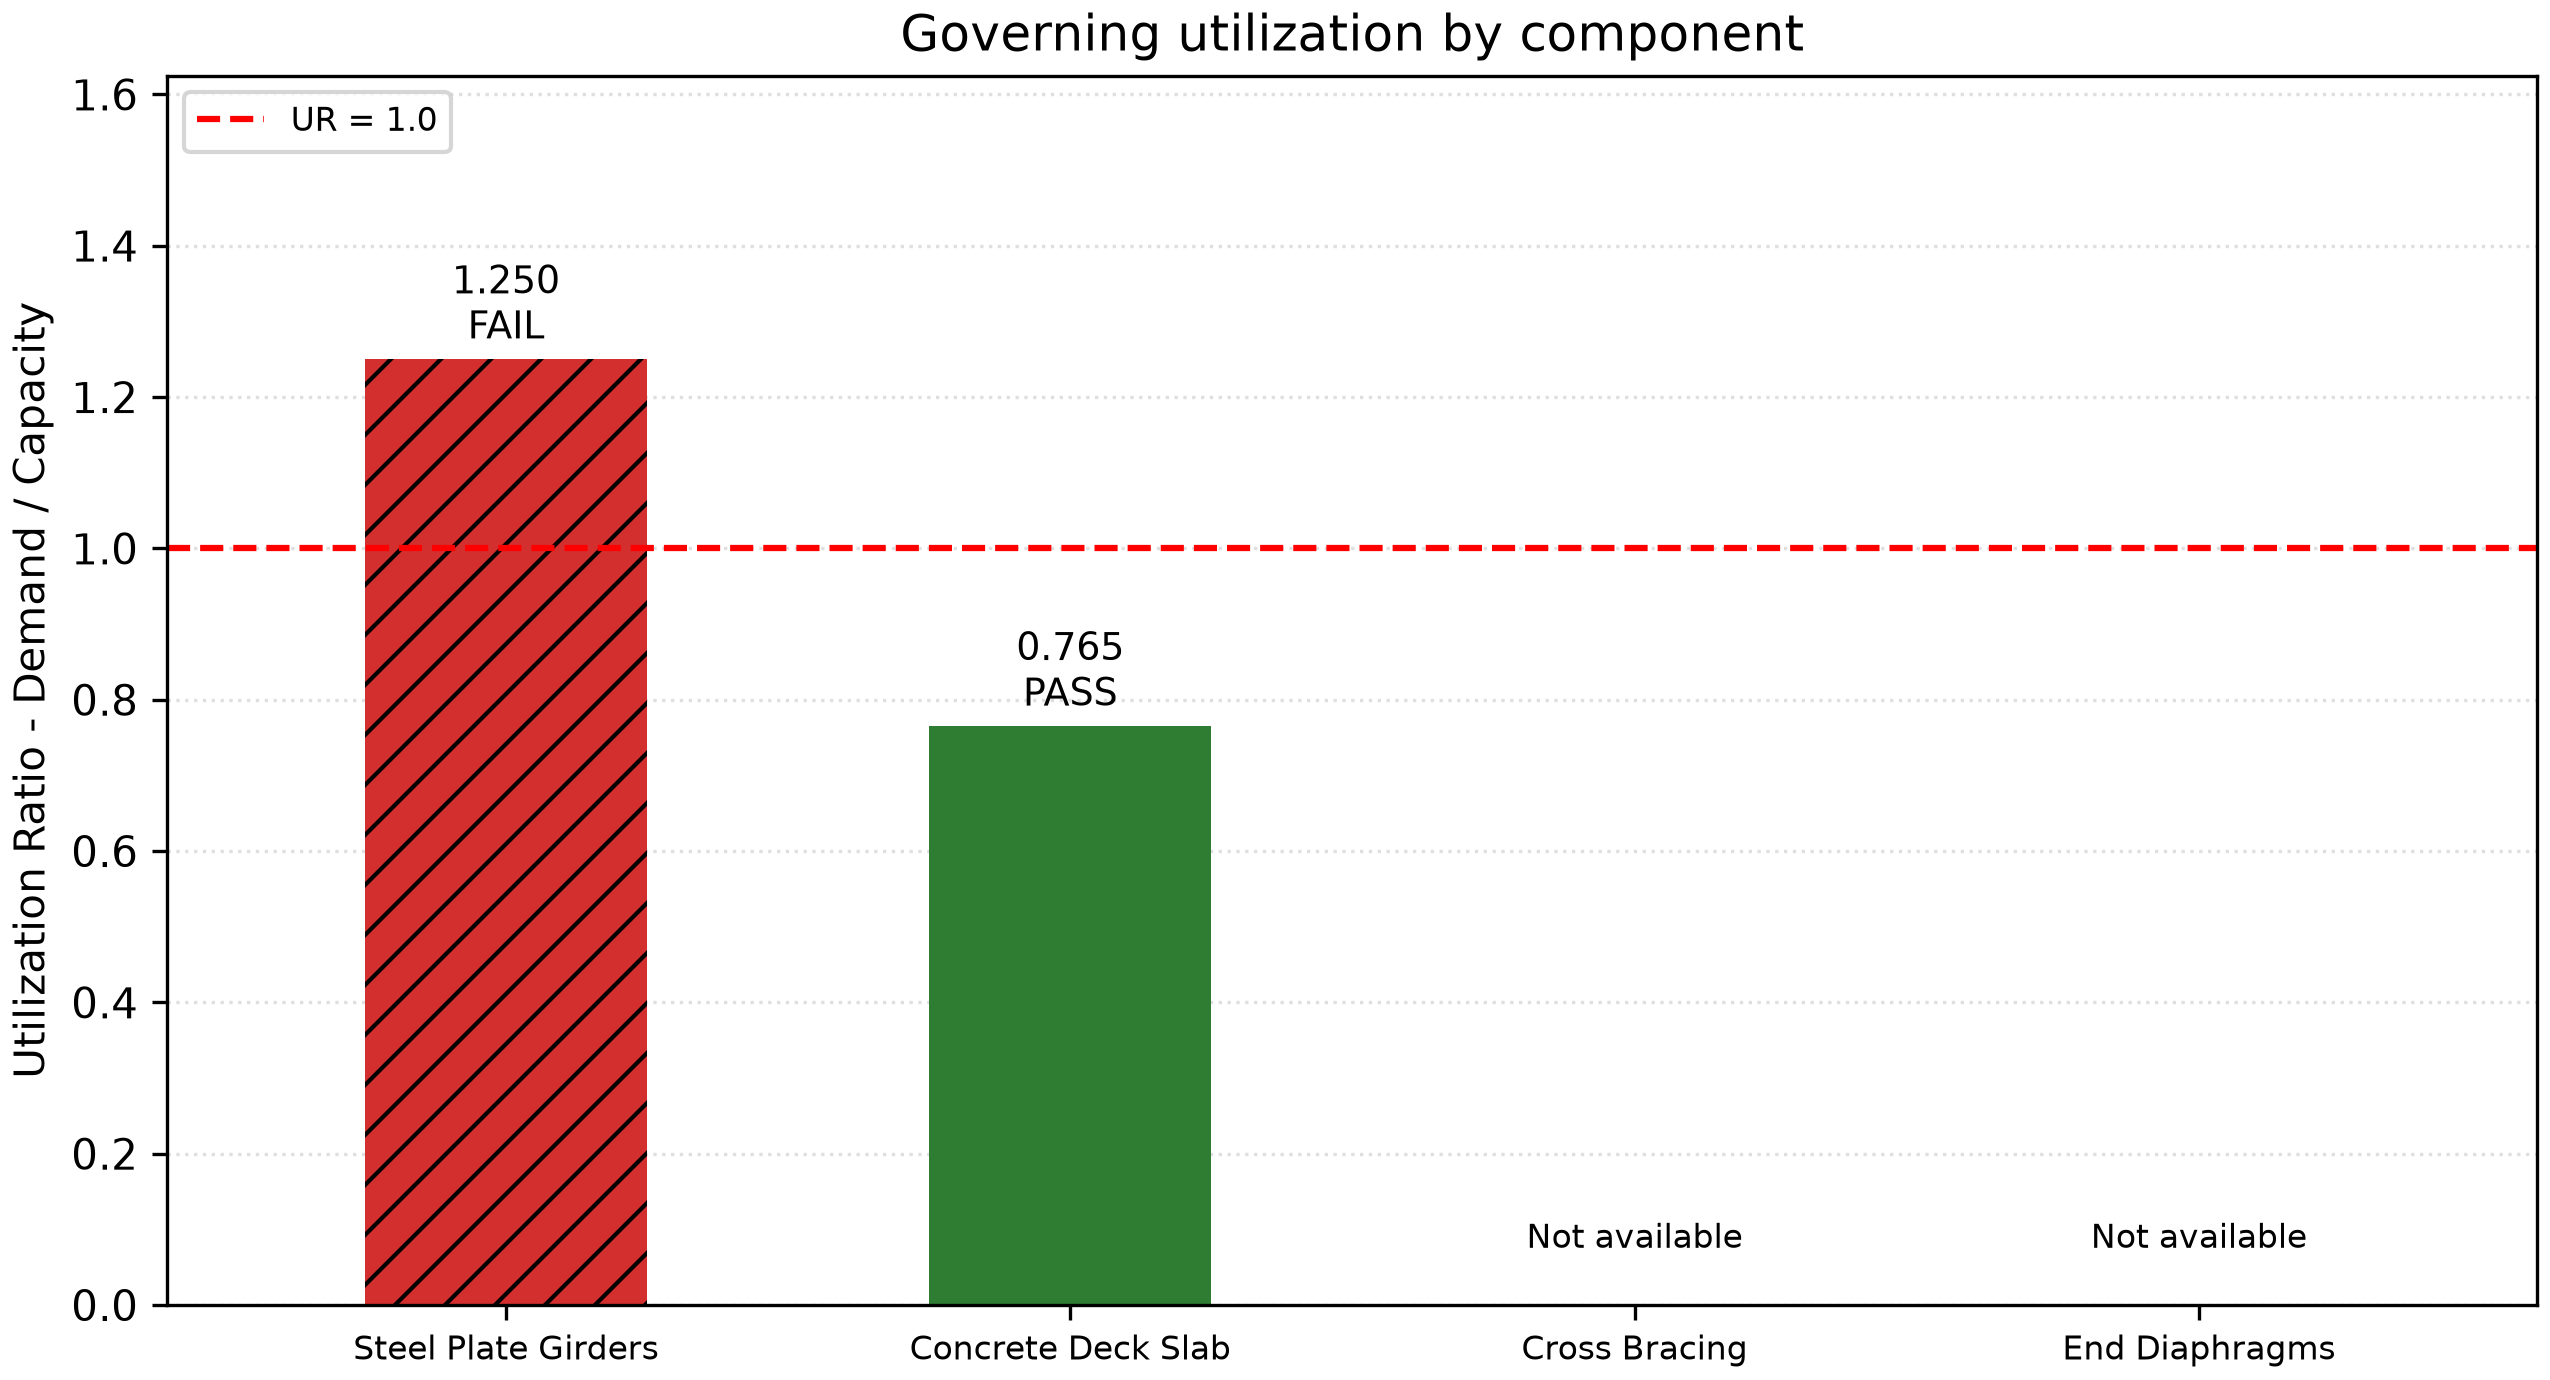
\includegraphics[width=0.92\linewidth,keepaspectratio]{images/ur_summary.png}
\caption{\textbf{Utilization Ratio (Demand / Capacity) Summary for Primary Bridge Elements (Steel Plate Girders, Concrete Deck Slab, Cross Bracing, End Diaphragms)}}
\label{fig:ur_summary}
\end{figure}

\vspace{1em}
\needspace{6\baselineskip}
\begin{longtable}{|C{\dimexpr0.241135\linewidth-2\tabcolsep-1.200000\arrayrulewidth\relax}|L{\dimexpr0.319149\linewidth-2\tabcolsep-1.200000\arrayrulewidth\relax}|C{\dimexpr0.163121\linewidth-2\tabcolsep-1.200000\arrayrulewidth\relax}|C{\dimexpr0.163121\linewidth-2\tabcolsep-1.200000\arrayrulewidth\relax}|>{\centering\arraybackslash}p{\dimexpr0.113475\linewidth-2\tabcolsep-1.200000\arrayrulewidth\relax}|}
\caption{\textbf{Overall Design Check Summary --- All Members}} \label{tab:overall_summary} \\
\hline
\rowcolor{tableHeaderBg} \textbf{Mem\-ber / Check} & \textbf{Governing Load Combo} & \textbf{Demand} & \textbf{Capacity} & \textbf{UR} \\[6pt]
\hline
\endfirsthead

\multicolumn{5}{c}{{\bfseries \tablename\ \thetable{} -- Continued from previous page}} \\[6pt]
\hline
\rowcolor{tableHeaderBg} \textbf{Mem\-ber / Check} & \textbf{Governing Load Combo} & \textbf{Demand} & \textbf{Capacity} & \textbf{UR} \\[6pt]
\hline
\endhead

\hline
\multicolumn{5}{r}{{\footnotesize \textit{Continued on next page\ldots}}} \\
\endfoot

\hline
\endlastfoot
Steel plate girders / G5 / Moment & Envelope & 125.000 kN-m & 100.000 kN-m & 1.250 (FAIL) \\[6pt]
\hline
Concrete deck slab / Deck / Flexure sagging & Basic ULS & 65.000 kN-m/m & 85.000 kN-m/m & 0.765 (PASS) \\[6pt]
\hline
Cross bracing / - / Backend result unavailable & Not available & Not available & Not available & Not available \\[6pt]
\hline
End diaphragms / - / Backend result unavailable & Not available & Not available & Not available & Not available \\[6pt]
\hline
\end{longtable}
\noindent\textit{Note: UR = Demand / Capacity. All values $\leq 1.0$ indicate passing checks. The governing check for each component is highlighted in the individual design check sections above.}


\chapter{Drawings and Visualizations}
\label{ch:drawings}

This section presents CAD-generated views of the designed bridge and its components. All views are generated automatically by OsdagBridge using pythonOCC.

\section{Bridge Configuration and Layout}
\label{sec:bridge-layout}

\begin{figure}[H]
\centering
\fbox{\parbox{0.97\textwidth}{
\textit{[ PLACEHOLDER:  Overall 3D Bridge Superstructure ]}
}}
\caption{Overall 3D Bridge Superstructure}
\label{fig:bridge-3d}
\end{figure}


\begin{figure}[H]
\centering
\fbox{\parbox{0.97\textwidth}{
\textit{[ PLACEHOLDER:  Typical Cross Section ]}
}}
\caption{Typical Cross Section}
\label{fig:cross-section}
\end{figure}


\begin{figure}[H]
\centering
\fbox{\parbox{0.97\textwidth}{
\textit{[ PLACEHOLDER:  Top View ]}
}}
\caption{Top View}
\label{fig:top-view}
\end{figure}


\section{Plate Girder --- Detailed Views}
\label{sec:girder-views}

\begin{figure}[H]
\centering
\fbox{\parbox{0.97\textwidth}{
\textit{[ PLACEHOLDER:  3D View of Plate Girders ]}
}}
\caption{3D View of Plate Girders}
\label{fig:girder-3d}
\end{figure}


\begin{figure}[H]
\centering
\fbox{\parbox{0.97\textwidth}{
\textit{[ PLACEHOLDER:  Cross Section of Plate Girder ]}
}}
\caption{Cross Section of Plate Girder}
\label{fig:girder-xsec}
\end{figure}


\begin{figure}[H]
\centering
\fbox{\parbox{0.97\textwidth}{
\textit{[ PLACEHOLDER:  Side View of Girder ]}
}}
\caption{Side View of Girder}
\label{fig:girder-side}
\end{figure}


\section{Cross Bracing Detail}
\label{sec:bracing-detail}

\begin{figure}[H]
\centering
\fbox{\parbox{0.97\textwidth}{
\textit{[ PLACEHOLDER:  Cross Bracing Layout ]}
}}
\caption{Cross Bracing Layout}
\label{fig:cb-layout}
\end{figure}


\noindent
\begin{minipage}[t]{0.31\textwidth}
\centering
\fbox{\parbox{0.95\linewidth}{\centering\textit{[ Cross Bracing -- Bracing Section ]}}}
\captionof{figure}{Cross Bracing -- Bracing Section}
\label{fig:cb-bracing-sec}
\end{minipage}
\hfill
\begin{minipage}[t]{0.31\textwidth}
\centering
\fbox{\parbox{0.95\linewidth}{\centering\textit{[ Cross Bracing -- Top Chord Section ]}}}
\captionof{figure}{Cross Bracing -- Top Chord Section}
\label{fig:cb-top-chord}
\end{minipage}
\hfill
\begin{minipage}[t]{0.31\textwidth}
\centering
\fbox{\parbox{0.95\linewidth}{\centering\textit{[ Cross Bracing -- Bottom Chord Section ]}}}
\captionof{figure}{Cross Bracing -- Bottom Chord Section}
\label{fig:cb-bottom-chord}
\end{minipage}


\section{End Diaphragm Detail}
\label{sec:diaphragm-detail}

\begin{figure}[H]
\centering
\fbox{\parbox{0.97\textwidth}{
\textit{[ PLACEHOLDER:  End Diaphragm Layout ]}
}}
\caption{End Diaphragm Layout}
\label{fig:ed-layout}
\end{figure}


\noindent
\begin{minipage}[t]{0.31\textwidth}
\centering
\fbox{\parbox{0.95\linewidth}{\centering\textit{[ End Diaphragm -- Bracing Section ]}}}
\captionof{figure}{End Diaphragm -- Bracing Section}
\label{fig:ed-bracing-sec}
\end{minipage}
\hfill
\begin{minipage}[t]{0.31\textwidth}
\centering
\fbox{\parbox{0.95\linewidth}{\centering\textit{[ End Diaphragm -- Top Chord Section ]}}}
\captionof{figure}{End Diaphragm -- Top Chord Section}
\label{fig:ed-top-chord}
\end{minipage}
\hfill
\begin{minipage}[t]{0.31\textwidth}
\centering
\fbox{\parbox{0.95\linewidth}{\centering\textit{[ End Diaphragm -- Bottom Chord Section ]}}}
\captionof{figure}{End Diaphragm -- Bottom Chord Section}
\label{fig:ed-bottom-chord}
\end{minipage}



\chapter{Material Take-off \& Quantity Summary}
\label{ch:material-takeoff}

This chapter details the comprehensive Bill of Materials (BOM) for all structural components, including structural steel (IS 2062), deck concrete (M40), reinforcement steel (Fe 500), and shear connector studs.

\vspace{1em}
\begingroup
\setlength{\tabcolsep}{4pt}
\renewcommand{\arraystretch}{1.18}
\begin{longtable}{|C{\dimexpr0.068493\linewidth-2\tabcolsep-1.142857\arrayrulewidth\relax}|L{\dimexpr0.260274\linewidth-2\tabcolsep-1.142857\arrayrulewidth\relax}|C{\dimexpr0.178082\linewidth-2\tabcolsep-1.142857\arrayrulewidth\relax}|C{\dimexpr0.123288\linewidth-2\tabcolsep-1.142857\arrayrulewidth\relax}|C{\dimexpr0.123288\linewidth-2\tabcolsep-1.142857\arrayrulewidth\relax}|C{\dimexpr0.123288\linewidth-2\tabcolsep-1.142857\arrayrulewidth\relax}|C{\dimexpr0.123288\linewidth-2\tabcolsep-1.142857\arrayrulewidth\relax}|}
\caption{\textbf{Bill of Materials (Steel, Concrete, and Reinforcement Quantities)}} \label{tab:bom} \\
\hline
\rowcolor{tableHeaderBg} \textbf{No.} & \textbf{Item Description} & \textbf{Vol.} & \textbf{Qty.} & \textbf{Total Volume} & \textbf{Wt. (MT)} & \textbf{Total Wt. (MT)} \\
\hline
\endfirsthead

\multicolumn{7}{c}{{\bfseries \tablename\ \thetable{} -- Continued from previous page}} \\[6pt]
\hline
\rowcolor{tableHeaderBg} \textbf{No.} & \textbf{Item Description} & \textbf{Vol.} & \textbf{Qty.} & \textbf{Total Volume} & \textbf{Wt. (MT)} & \textbf{Total Wt. (MT)} \\
\hline
\endhead

\hline
\multicolumn{7}{r}{{\footnotesize \textit{Continued on next page\ldots}}} \\
\endfoot

\hline
\endlastfoot

1 & Structural Steel (IS 2062) for Girders & $0.03492\text{ m}^2 \times 30.00\text{ m} = 1.04756\text{ m}^3$ & 5 & 5.24 & 8.22 & 41.12 \\
\hline
2(a) & Cross Bracing - Top Chord & N.A. & N.A. & N.A. & N.A. & N.A. \\
\hline
2(b) & Cross Bracing - Bottom Chord & N.A. & N.A. & N.A. & N.A. & N.A. \\
\hline
2(c) & Cross Bracing - Diagonal Chord & N.A. & N.A. & N.A. & N.A. & N.A. \\
\hline
3 & Concrete (M40) for Deck Slab & $12.15\text{ m} \times 0.25\text{ m} \times 30.00\text{ m} = 91.12\text{ m}^3$ & 1 & 91.12 & 227.81 & 227.81 \\
\hline
4 & Reinforcement Steel (Fe 500) & $0.046433\text{ m}^2 \times 30.00\text{ m} = 1.39299\text{ m}^3$ & 1 & 1.39 & 10.93 & 10.93 \\
\hline
5 & Shear Stud Connectors & N.A. & N.A. & N.A. & N.A. & N.A. \\
\hline
6 & Crash Barrier & $0.30228\text{ m}^2 \times 30.00\text{ m} = 9.06848\text{ m}^3$ & 2 & 18.14 & 22.67 & 45.34 \\
\hline
\end{longtable}
\endgroup
\noindent\textit{Reinforcement weight is an estimate using 120 kg per cubic metre of concrete. End-diaphragm quantity is not available from the backend.}

\vspace{1.5em}
\begin{figure}[H]
\centering
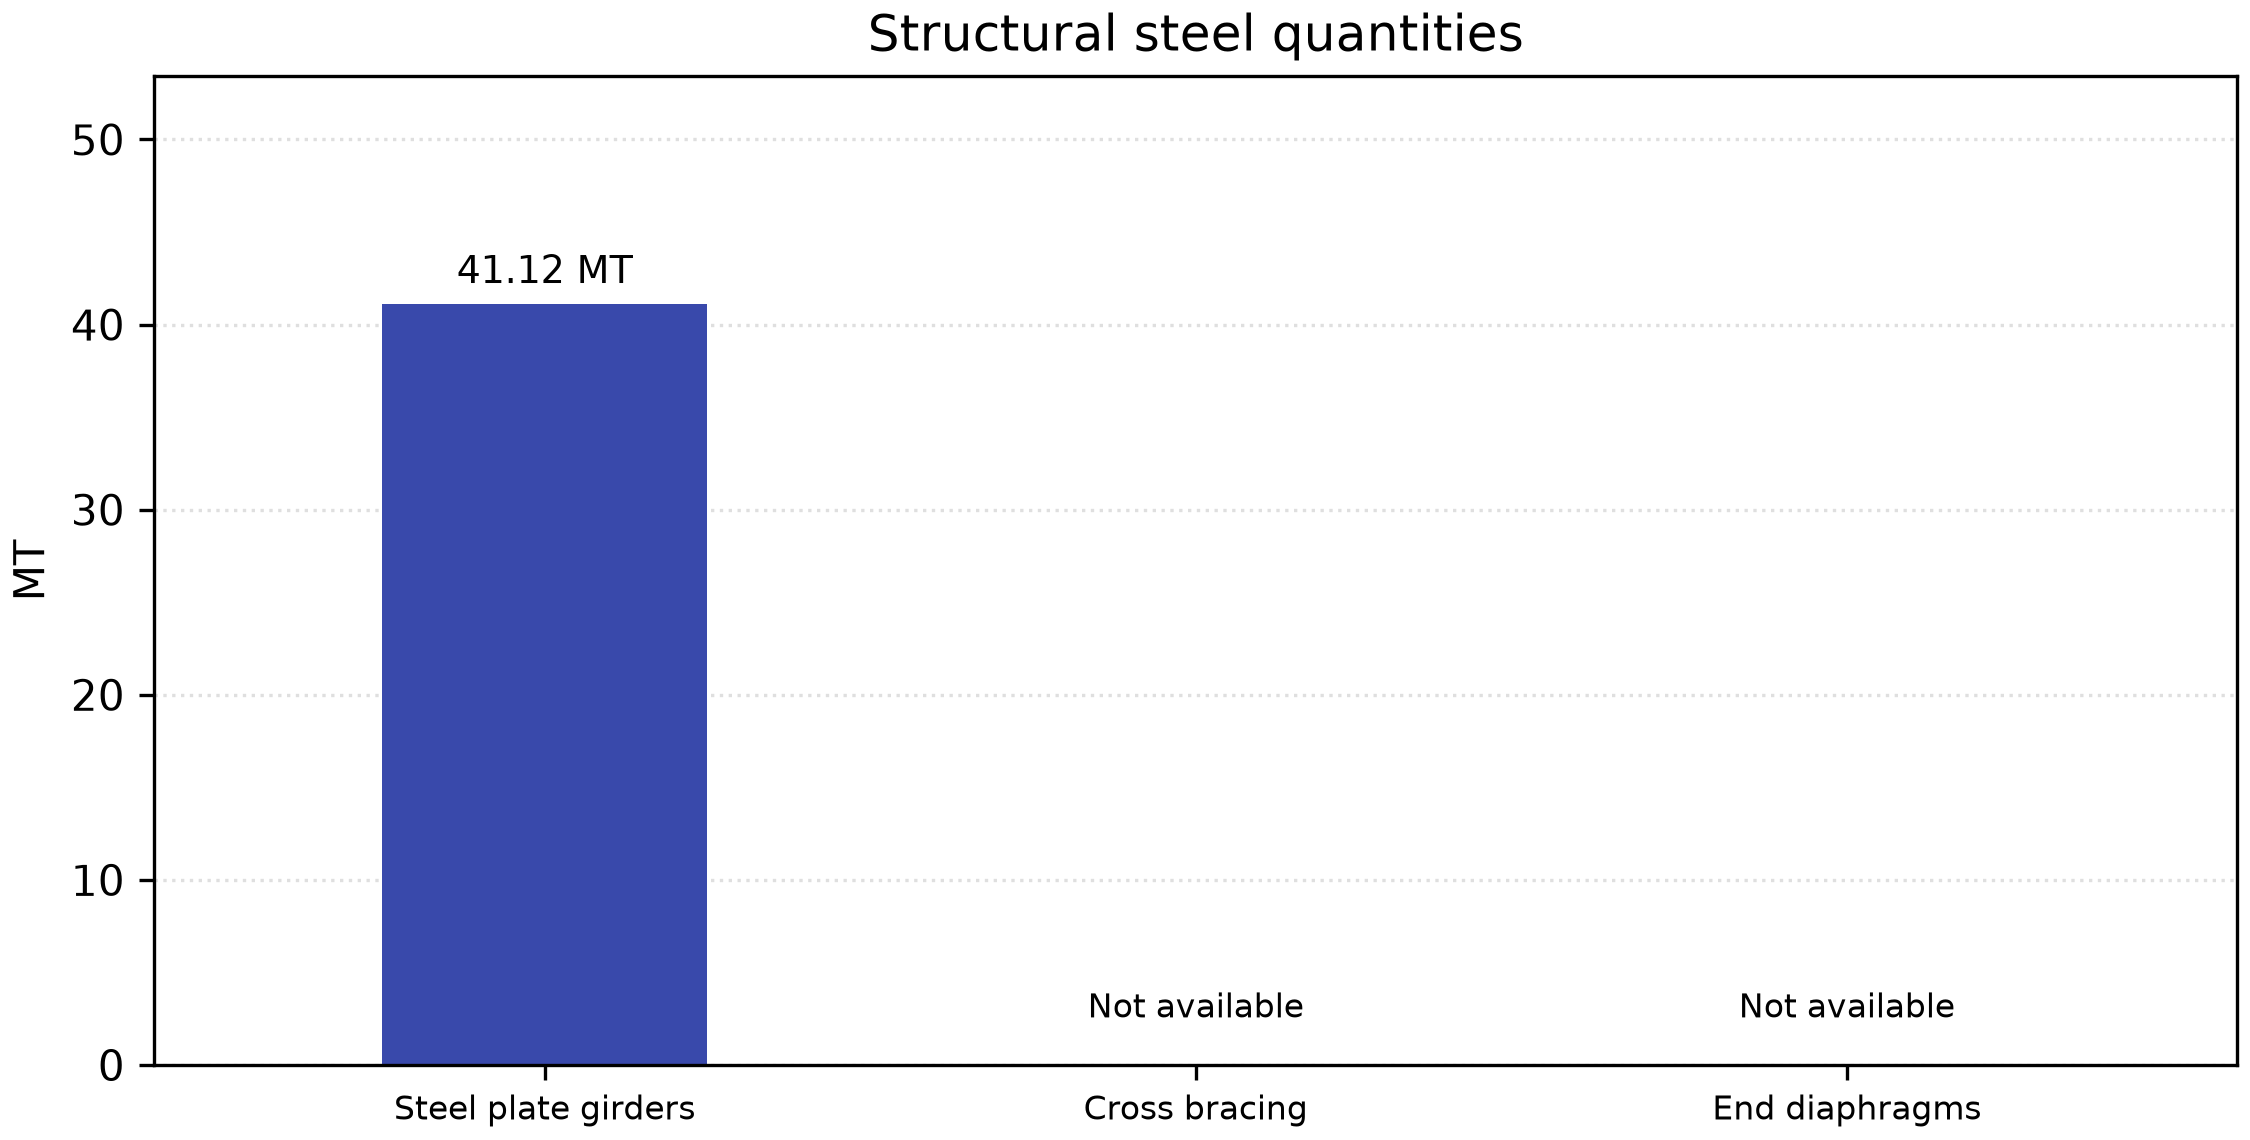
\includegraphics[width=0.88\linewidth,keepaspectratio]{images/material_steel_tonnage.png}
\caption{\textbf{Structural Steel Tonnage Breakdown by Component (MT) --- Girders, Cross Bracing, End Diaphragms}}
\label{fig:steel_tonnage}
\end{figure}

\vspace{1.0em}
\begin{figure}[H]
\centering
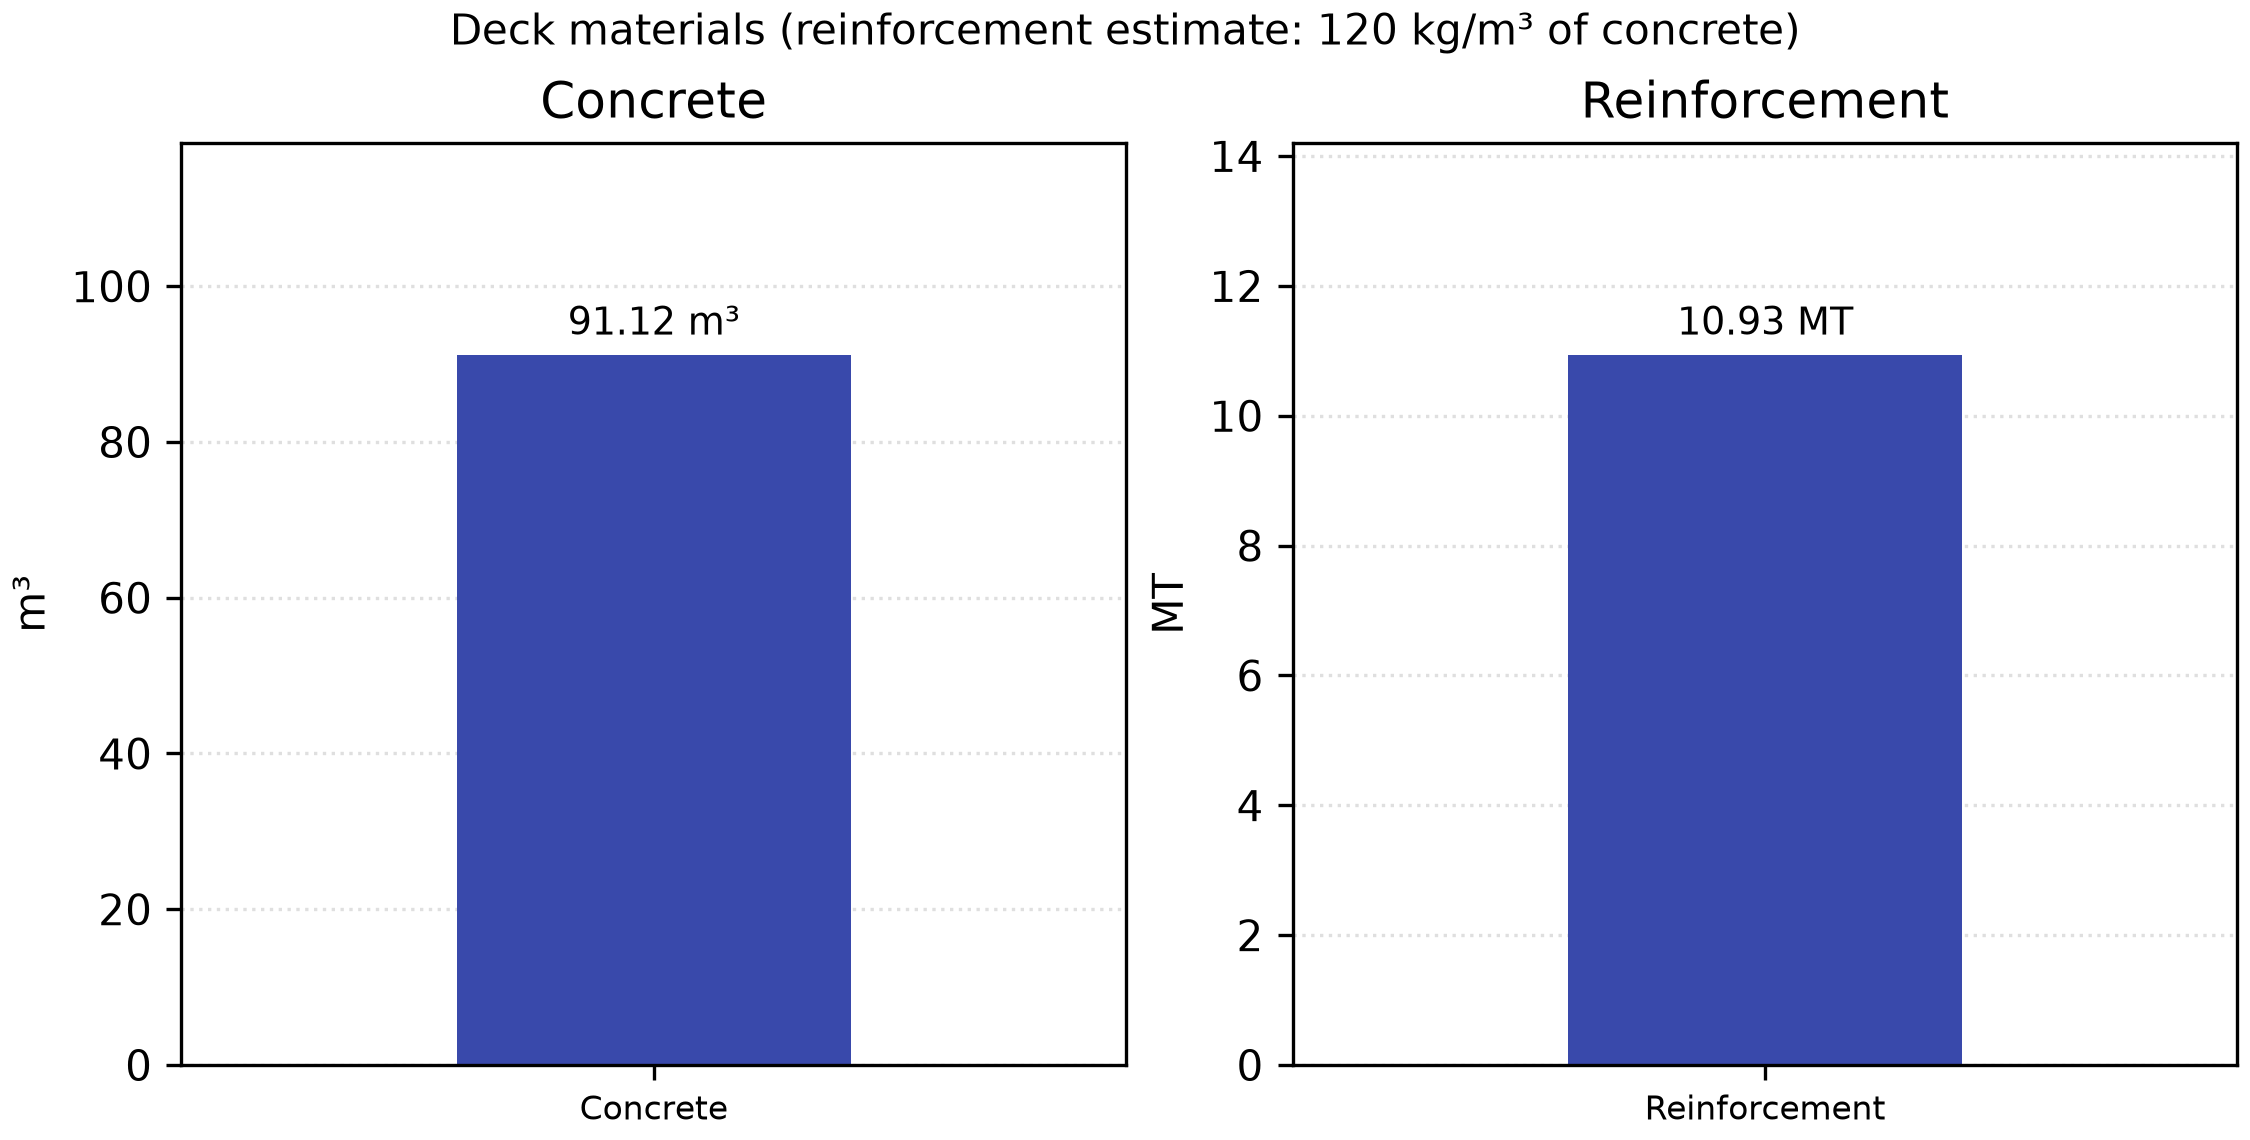
\includegraphics[width=0.85\linewidth,keepaspectratio]{images/material_concrete_rebar.png}
\caption{\textbf{Primary Deck Materials: Concrete Volume ($m^3$) vs. Reinforcement Steel Weight (MT) Take-off}}
\label{fig:concrete_rebar}
\end{figure}


\chapter{Standards \& Assumptions}
\label{ch:Design Standards}

This section provides references to standards used to calibrate the OsdagBridge
design modules, and notes the limitations of the current software version.

\section{Design Standards}
\label{sec:design_standards}

The following Indian Road Congress (IRC) codes and Indian Standards (IS)
form the basis of all design calculations in this software.

\vspace{0.5cm}

\begin{longtable}{|C{\dimexpr0.156250\linewidth-2\tabcolsep-1.333333\arrayrulewidth\relax}|C{\dimexpr0.125000\linewidth-2\tabcolsep-1.333333\arrayrulewidth\relax}|L{\dimexpr0.718750\linewidth-2\tabcolsep-1.333333\arrayrulewidth\relax}|}
\caption{\textbf{IRC Codes}} \label{tab:irc_codes} \\
\hline
\rowcolor{tableHeaderBg} \textbf{Code} & \textbf{Year} & \textbf{Title / Scope} \\
\hline
\endfirsthead

\multicolumn{3}{c}{{\bfseries \tablename\ \thetable{} -- Continued from previous page}} \\[6pt]
\hline
\rowcolor{tableHeaderBg} \textbf{Code} & \textbf{Year} & \textbf{Title / Scope} \\
\hline
\endhead

\hline
\multicolumn{3}{r}{{\footnotesize \textit{Continued on next page\ldots}}} \\
\endfoot

\hline
\endlastfoot

IRC 5 & 2015 & General Features of Design - carriageway widths, kerb, footpath dimensions \\[6pt]
\hline
IRC 6 & 2017 & Loads and Load Combinations - dead load, live load, impact, wind, temperature, etc. \\[6pt]
\hline
IRC 22 & 2015 & Composite Construction (LS) - Composite section properties, ULS/SLS design, shear connectors \\[6pt]
\hline
IRC 24 & 2010 & Steel Road Bridges (LS) - Stiffener design, skew angle limits, diaphragm requirements \\[6pt]
\hline
IRC 112 & 2020 & Concrete Road Bridges - Deck slab flexure, shear, crack width, reinforcement \\[6pt]
\hline
IRC SP 114 & 2018 & Seismic Design of Road Bridges \\[6pt]
\hline
\end{longtable}

\vspace{1em}

\begin{longtable}{|C{\dimexpr0.156250\linewidth-2\tabcolsep-1.333333\arrayrulewidth\relax}|C{\dimexpr0.125000\linewidth-2\tabcolsep-1.333333\arrayrulewidth\relax}|L{\dimexpr0.718750\linewidth-2\tabcolsep-1.333333\arrayrulewidth\relax}|}
\caption{\textbf{IS Codes}} \label{tab:is_codes} \\
\hline
\rowcolor{tableHeaderBg} \textbf{Code} & \textbf{Year} & \textbf{Scope} \\
\hline
\endfirsthead

\multicolumn{3}{c}{{\bfseries \tablename\ \thetable{} -- Continued from previous page}} \\[6pt]
\hline
\rowcolor{tableHeaderBg} \textbf{Code} & \textbf{Year} & \textbf{Scope} \\
\hline
\endhead

\hline
\multicolumn{3}{r}{{\footnotesize \textit{Continued on next page\ldots}}} \\
\endfoot

\hline
\endlastfoot

IS 800 & 2007 & Steel construction - tension, compression, bending, shear, LTB, stiffeners, combined checks \\[6pt]
\hline
IS 456 & 2000 & Concrete - simplified stress-block for deck moment capacity \\[6pt]
\hline
IS 1786 & 2008 & Reinforcement steel properties \\[6pt]
\hline
IS 1893 (Part 3) & 2014 & Earthquake resistant design \\[6pt]
\hline
IS 2062 & 2011 & Structural steel - yield and ultimate strength by grade \\[6pt]
\hline
\end{longtable}

\clearpage
\section{Analysis and Design Assumptions of This Version}
\label{sec:ch8_assumptions}

\textbf{Structural Analysis}

\begin{itemize}
    \item All girders are modelled as simply supported; continuous spans are not currently supported.
    \item A 3D grillage model (OSPGrillage) is used for load distribution. Grillage members carry composite section properties after the construction stage.
    \item The transverse member forces are computed using an approximate 2D frame analogy. For irregular or skewed geometries, a 3D FEM is recommended.
    \item Fixed bearing stiffness is modelled as $k = 1{,}000{,}000 \,\text{kN/m}$ (virtually rigid); free/expansion bearing as $k = 100 \, \text{kN/m}$.
    \item Construction stage sequence analysis is approximate. Detailed staged analysis should be performed for long-term deflection checks.
\end{itemize}

\textbf{Composite Action}

\begin{itemize}
    \item Full shear connection is assumed at ULS with headed stud connectors designed per IRC 22:2015 Cl.606.
    \item Short-term composite section properties (modular ratio $n = E_s/E_{cm}$) are used for ULS checks.
    \item Long-term composite section properties (with creep-adjusted modular ratio) are used for SLS deflection and crack-width checks.
    \item Pre-composite stage: the steel girder alone resists all construction loads prior to concrete gaining strength.
\end{itemize}


\textbf{Material Properties (IRC 22:2015 Annex III)}

\begin{itemize}
\item Steel: $E_s = 200{,}000 \, \text{MPa}, \ G_s = 80{,}000 \, \text{MPa}, \ \nu = 0.30, \ \alpha = 11.7 \times 10^{-6}/^\circ\mathrm{C}$ (grade-independent).
\item Minimum structural concrete grade: M25.
\item Default reinforcement grade: Fe500.
\end{itemize}

\textbf{Partial Safety Factors (IRC 22:2015 Cl.601.4)}

\begin{itemize}
\item $\gamma_{m0}$ (steel yield, ULS) = 1.10
\item $\gamma_{m1}$ (steel ultimate, ULS) = 1.25
\item Reinforcement (ULS) = 1.15
\item Welds -- shop: 1.25; field: 1.50
\item Fatigue ($\gamma_{mft}$) = 1.35
\end{itemize}

\textbf{Loading}

\begin{itemize}
\item Dead load densities per IRC 6:2017 Cl.203: structural steel $78.5 \ \text{kN/m}^3$, concrete $25.0 \ \text{kN/m}^3$, bituminous wearing course $24.0 \ \text{kN/m}^3$.
\item Multi-lane live load reduction factors per IRC 6:2017 Cl.204.4 Table 6A: 1st lane = 1.0, 2nd lane = 0.8, 3rd lane onwards = 0.4.
\item Impact factor (dynamic load allowance) computed from span per IRC 6:2017 Cl.208.2/\allowbreak 208.3.
\item Wind load applied as transverse, longitudinal, and vertical components per IRC 6:2017 Cl.209.3.3--209.3.5.
\end{itemize}

\textbf{Serviceability Limits}

\begin{itemize}
\item Deflection limits (IRC 22:2015 Cl.604.3.2): live load + impact $\leq L/800$; total $\leq L/600$.
\item SLS stress limits: concrete $\sigma_c \leq 0.48 f_{ck}$; rebar $\sigma_s \leq 0.80 f_{yk}$; steel $f_e \leq 0.9 f_y$.
\item Permissible crack width: $w_k \leq 0.3 \ \text{mm}$ (bridge deck, exposure class XS2/XD2 per IRC 112:2020 Cl.12.3.2).
\end{itemize}

\textbf{Fatigue}

\begin{itemize}
\item Reference fatigue life: $N_{sc} = 2 \times 10^6$ cycles (IRC 22:2015 Cl.605).
\item Constant stress range is assumed. A thickness correction factor $\mu_r$ is applied for plate thickness $> 25 \ \text{mm}$.
\end{itemize}

\textbf{Stiffener Design}

\begin{itemize}
\item Intermediate transverse stiffener and bearing stiffener design follows IS 800:2007 Cl.8.7.2/8.7.3 and IRC 24:2010 Cl.509.7.2/509.7.3.
\end{itemize}


\section{Known Limitations of This Version}
\label{sec:limitations}

\begin{itemize}
\item Substructure (piers, pile caps, foundations) and bearing design are not included.
\item Splice connection design is not implemented.
\item Skew angle $>$ 15 degrees requires independent manual analysis (IRC 24 Cl. 504.8).
\item Construction stage sequence analysis is approximate; detailed staged analysis
  should be performed for long-term deflection checks.
\item The grillage analysis assumes simply supported boundary conditions;
  continuous spans are not currently supported.
\end{itemize}


\chapter*{References}
\addcontentsline{toc}{chapter}{References}


\begin{enumerate}

\item IRC 5 (2024) --- \textit{Standard Specifications and Code of Practice for Road Bridges, Section I: General Features of Design.}

\item IRC 6 (2017) --- \textit{Standard Specifications and Code of Practice for Road Bridges, Section II: Loads and Load Combinations.}

\item IRC 22 (2014) --- \textit{Standard Specifications and Code of Practice for Road Bridges, Section VI: Composite Construction (Limit State Design).}

\item IRC 24 (2010) --- \textit{Standard Specifications and Code of Practice for Road Bridges, Section V: Steel Road Bridges (Limit State Method).}

\item IRC 112 (2011) --- \textit{Code of Practice for Concrete Road Bridges.}

\item IRC SP 114 (2018) --- \textit{Guidelines for Seismic Design of Road Bridges.}

\item IS 800 (2007) --- \textit{Indian Standard: General Construction in Steel --- Code of Practice.}

\item IS 2062 (2011) --- \textit{Hot Rolled Medium and High Tensile Structural Steel --- Specification.}

\item Subramanian, N. (2008). \textit{Design of Steel Structures.} Oxford University Press.

\item Steel-INSDAG Teaching Resource Materials. \url{https://www.steel-insdag.org}

\end{enumerate}

\end{document}
